\section{Control File}
\subsection{Overview of Control File}
These listed model features are denoted in the control file in the following order:
	\begin{enumerate}
		\item Number of growth patterns and platoons
		\item Design matrix for assignment of recruitment to area/settlement event/growth pattern
		\item Design matrix for movement between areas
		\item Definition of time blocks that can be used for time-varying parameters
		\item Controls far all time-varying parameters
		\\
		\item Specification for growth and fecundity
		\item Natural mortality growth parameters, weight-at-length, maturity, and fecundity, for each sex 
		\item Hermaphroditism parameter line (if used)
		\item Recruitment distribution parameters for each area, settlement event, and growth pattern
		\item Cohort growth deviation
		\item Movement between areas (if used)
		\item Age error parameter line (if used)
		\item Catch multiplier (if used)
		\item Fraction female 
		\item Setup for any mortality-growth parameters are time-varying
		\item Seasonal effects on biology parameters
		\\
		\item Spawner-recruitment parameters
		\item Setup for any stock recruitment parameters are time-varying
		\item Recruitment deviations
		\\
		\item F ballpark value in specified year
		\item Method for calculating fishing mortality (F)
		\item Initial equilibrium F for each fleet
		\\
		\item Catchability (Q) setup for each fleet and survey
		\item Catchability parameters
		\item Setup for any catchability parameters are time-varying
		\\
		\item Length selectivity, retention, discard mortality setup for each fleet and survey
		\item Age selectivity setup for each fleet and survey
		\item Parameters for length selectivity, retention, discard mortality for each fleet and survey
		\item Parameters for age selectivity, retention, discard mortality for each fleet and survey
		\item Setup for any selectivity parameters that are time-varying
		\\
		\item Tag-recapture parameters
		\\
		\item Variance adjustments
		\item Lambdas for likelihood components
	\end{enumerate}
The order in which they appear in the control file has grown over time rather opportunistically, so it may not appear particularly logical at this time, especially various aspects of recruitment distribution and growth.  When the same information is entered via the SS GUI, it is organized more logically and then written in this form to the text control file.

\subsection{Parameter Line Elements}
The primary role of the SS control file is to define the parameters to be used by the model.  The general syntax of the 14 elements of a long parameter line is described here.  If used, time-varying parameter lines use only the first seven elements of a parameter line and will be referred to as a short parameter line.  Three types of time-varying properties can be applied to a base parameter:  blocks or trend, environmental linkage, and random deviation.  Each parameter line contains:

\hypertarget{Priors}{} \hypertarget{paraOrder}{}
\begin{center}
	\begin{tabular}{p{2cm} p{3cm} p{10cm}}
		\hline
		Column & Element & Description \Tstrut\Bstrut\\
		\hline
		1 & LO & Minimum value for the parameter\Tstrut\\
		2 & HI & Maximum value for the parameter\Tstrut\\
		3 \Tstrut & INIT & Initial value for the parameter. If the phase (described below) for the parameter is negative the parameter is fixed at this value. If the ss.par file is read, it overwrites these INIT values.\\
		4 \Tstrut & PRIOR & Expected value for the parameter.  This value is ignored if the prior type is 0 (no prior) or 1 (symmetric beta). If the selected prior type (described below) is lognormal, this value is entered in log space. \\
		5 \Tstrut & PRIOR SD & Standard deviation for the prior, used to calculate likelihood of the current parameter value. This value is ignored if prior type is 0.\\
		6 \Tstrut & \hyperlink{PriorDescrip}{PRIOR TYPE}  & 0 = none, \\
		& & 1 = symmetric beta; \\
		& & 2 = full beta; \\
		& & 3 = lognormal without bias adjustment; \\
		& & 4 = lognormal with bias adjustment; \\
		& & 5 = gamma; and \\
		& & 6 = normal. \\
		7 \Tstrut & PHASE & Phase in which parameter begins to be estimated.  A negative value causes the parameter to retain its INIT value (or value read from the ss.par file).\Bstrut\\
		8  \Tstrut & Env var \& Link & Create a linkage to an input environmental time-series\\
		9  \Tstrut & Dev link & Invokes use of the deviation vector in the linkage function \\
		10 \Tstrut & Dev min yr & Beginning year for the deviation vector \\
		11 \Tstrut & Dev max yr & Ending year for the deviation vector\\
		12 \Tstrut & Dev phase & Phase for estimation for elements in the deviation vector \\
		13 \Tstrut & Block & Time block or trend to be applied \\
		14 \Tstrut & Block function & Functional form for the block offset. \Bstrut\\
		\hline
	\end{tabular}
\end{center}

Note that relative to SS v.3.24,  the order of PRIOR SD and PRIOR TYPE have been switched and the PRIOR TYPE options have been renumbered.

The full parameter line (14 in length) syntax for the mortality-growth, spawn-recruitment, catchability, and selectivity sections provides additional controls to give the parameter time-varying properties.  If a parameter (a full parameter line of length 14) is set up to be time-varying (i.e., parameter time blocks, annual deviations), short parameter lines, the first 7 elements, are required to be specified immediately after the main parameter block (i.e., mortality-growth parameter section).  Additional information regard time-varying parameters and how to implement them in SS is available \hyperlink{tvOrder}{below}, with in depth information provided in the \hyperlink{TVpara}{Using Time-Varying Parameters} section.


\subsection{Terminology}
The term COND appears in the "Typical Value" column of this documentation (it does not actually appear in the model files), it indicates that the following section is omitted except under certain conditions, or that the factors included in the following section depend upon certain conditions. In most cases, the description in the definition column is the same as the label output to the ss\_new files.

\subsection{Beginning of Control File Inputs}
\begin{center}
	\begin{longtable}{p{0.5cm} p{2cm} p{12cm}}
		\hline
		\multicolumn{2}{l}{Typical Value} & Description and Options\Tstrut\Bstrut\\
		\hline
		\endfirsthead

		\hline
		\multicolumn{2}{l}{Typical Value} & Description and Options\Tstrut\Bstrut\\
		\hline
		\endhead

		\hline
		\endfoot

		\endlastfoot

		\multicolumn{2}{l}{\#C comment }\Tstrut & Comments beginning with \#C at the top of the file will be retained and included in output. \Bstrut\\
		\hline

		0 & & 0 = Do not read the weight-at-age (wtatage.ss) file; \Tstrut\\
		  & & 1 = Read the weight-at-age (wtatage.ss) file, also read and use the growth parameters; and \\
		  & & 2 = Future option to read the weight-at-age (wtatage.ss) file, then omit reading and using growth parameters and all length-based data.\\
		  & & Additional information on the weight-at-age file and the expected formatting can be found in the \hyperlink{WAA}{Empirical Weight-at-Age}  section.\Bstrut\\

		%\hline
		\pagebreak
		1 & & Number (N) of growth patterns (GP), also referred to as morphs:\Tstrut\\
		& & These are collections of fish with unique biological characteristics (growth, mortality, weight-length, reproduction). The GP x Sex x Settlement Events constitute unique growth patterns that are tracked in SS. They are assigned these characteristics at birth and retain them throughout their lifetime. At recruitment, growth pattern members are distributed across areas (if any) and they retain their biological characteristics even if they move to another area in which a different cohort with different biological characteristics might predominate.  For example, one could assign a fast-growing growth pattern to recruit predominately in a southern areas and a slow-growing growth pattern to a northern area. The natural mortality and growth parameters are specified for each growth pattern in the mortality-growth parameter section in the order of females growth pattern 1 to growth pattern N followed by males growth pattern 1 to growth pattern N in a two sex model.\Bstrut\\

		\hline
		1 & & Number of platoons within a growth pattern/morph:\Tstrut\\
		& & This allows exploration of size-dependent survivorship. A value of 1 will not create additional platoons.  Odd-numbered values (i.e., 3, 5) will break the overall morph into that number of platoons creating a smaller, larger, and mean growth platoon.  The higher the number of platoons the slower SS will run, so values above 5 not advised.  The fraction of each morph assigned to each platoon is custom-input or designated to be a normal approximation.  When multiple platoons are designated, an additional input is the ratio of between platoon to within platoon variability in size-at-age.  This is used to partition the total growth variability.  For the platoons, their size-at-age is calculated as a factor (determined from the between-within variability calculation) times the size-at-age of the central morph which is determined from the growth parameters for that Growth Pattern x Sex. \Bstrut\\

		\multicolumn{2}{l}{COND > 1}& \multicolumn{1}{l}{\parbox{12cm}{Following 2 lines are conditional on N platoons > 1.}} \Tstrut\Bstrut\\

		& 0.7 & Platoon between/within standard deviation ratio. Ratio of the amount of variability in length-at-age between platoons to within platoons.\Bstrut\\

		& 0.2 0.6 0.2 & Distribution among platoons. Enter either a custom vector or enter a vector of length N with the first value of -1 to get a normal approximation: (0.15, 0.70, 0.15) for 3 platoons, or 5 platoons (0.031, 0.237, 0.464, 0.237, 0.031).\Bstrut\\
		\hline
	\end{longtable}
\end{center}

\subsubsection{Weight-at-Age}
SS added the capability to read empirical body weight-at-age for the population and each fleet, starting in version 3.04, in lieu of generating these weights internally from the growth parameters, weight-at-length, and size-selectivity. The values are read from a separate file named, wtatage.ss. This file is only required to exist if this option is selected.  See the \hyperlink{WAA}{Empirical Weight-at-Age} section for additional information on file formatting for empirical weight-at-age.

\subsubsection{Settlement Timing for Recruits and Distribution}
In older versions of SS one value of spawning biomass was calculated annually at the beginning of one specified spawning season and this spawning biomass produced one annual total recruitment value. The annual recruitment value was then distributed among seasons, areas, and growth types according to other model parameters.

Additional control of the seasonal timing was added in SS v.3.30 and now there now is an explicit elapsed time between spawning and recruitment. Spawning still occurs, just once per year, which defines a single spawning biomass for the stock-recruitment curve but its timing can be at any specified time, not just the beginning of a season.  Recruitment of the progeny from an annual spawning can now enter the population in one or more settlement events, at some point after spawning as defined by the user.  

	
\begin{longtable}{p{1.25cm} p{1.25cm} p{1cm} p{11cm}}
		\hline
		\multicolumn{2}{l}{Typical Value} & \multicolumn{2}{l}{Description and Options}\Tstrut\Bstrut\\
		\hline
		\endfirsthead
		
		\hline
		\multicolumn{2}{l}{Typical Value} & \multicolumn{2}{l}{Description and Options}\Tstrut\Bstrut\\
		\hline
		\endhead
		
		\hline
		\endfoot
		
		\endlastfoot
		
		1 \Tstrut & &\multirow{2}{4cm}[-0.1cm]{\parbox{12cm}{Recruitment distribution method. This section controls which combinations of growth pattern x area x settlement will get a portion of the total recruitment coming from each spawning.  Options:}} \\ \\ 
		& & \multirow{2}{4cm}[-0.1cm]{\parbox{12cm}{1 = no longer available (used the SS v.3.24 or earlier setup);}} \\
		& & \multirow{2}{4cm}[-0.1cm]{\parbox{12cm}{2 = main effects for growth pattern, settle timing, and area;}} \\
		& & \multirow{2}{4cm}[-0.1cm]{\parbox{12cm}{3 = each settle entity; and}} \\
		& & \multirow{2}{4cm}[-0.1cm]{\parbox{12cm}{4 = none, no parameters (only if growth pattern x settlement x area = 1).}} \Bstrut\\
		
		\hline
		1 & & \multicolumn{2}{l}{Spawner-Recruitment (not implement yet, but required), options:} \Tstrut\\
		& & \multicolumn{2}{l}{1 = global; and}\\
		& & \multirow{2}{4cm}[-0.1cm]{\parbox{12cm}{2 = by area (by area is not yet implemented; there is a conceptual challenge to doing the equilibrium calculation when there is fishing).}}\Bstrut\\\\
		
		\hline
		1 \Tstrut & & \multirow{2}{4cm}[-0.1cm]{\parbox{12cm}{Number of recruitment settlement assignments.  Must be at least 1 even if only 1 settlement and 1 area because the timing of that settlement must be specified.}}\Bstrut\\\\\\
		
		\hline
		0 \Tstrut & & \multicolumn{2}{l}{Future feature, not implement yet but required.} \Bstrut\\
		
		\hline
		Growth Pattern & Month & Area  & Age at settlement \Tstrut \\
		\hline
		1 & 5.5 & 1 & 0 \Bstrut\\
		\hline
\end{longtable} 

The above example specifies settlement to mid-May (month 5.5). Note that normally the calendar age at settlement is 0 if settlement happens between the time of spawning and the end of that year, and at age 1 if settlement is in the year after spawning. 

Below is an example set-up where there are multiple settlement events, with one occurring the following year after spawning: 
\begin{center}
	\begin{tabular}{p{3cm} p{2cm} p{2cm} p{7cm}}
		\hline
		3 & \multicolumn{3}{l}{Number of recruitment settlement events}\Tstrut\\
		0 & \multicolumn{3}{l}{Unused option}\Bstrut\\
		\hline
		Growth Pattern & Month & Area & Age (for each settlement assignment)\Tstrut\Bstrut\\
		\hline
		1 & 11.0 & 1 & 0 \Tstrut\\
		1 & 12.0 & 1 & 0 \\
		1 & 1.0  & 1 & 1 \Bstrut\\
		\hline
	\end{tabular}		
\end{center}

%\myparagraph{Recruitment Timing and Settlement}
Details regarding settlement of recruits and  timing:
	\begin{itemize}
		\item Recruitment happens in specified settlement events (growth pattern, month, area).
		\item Number of unique settlement timings is calculated at runtime.
		\item Now there is explicit elapsed time between spawning and recruitment.
		\item Growth and natural mortality of the platoon begins at time of settlement, which is its real age 0.0 for growth; but pre-settlement fish exist from the beginning of the season of settlement, so can be caught if selected.
		\item Age at recruitment now user-controlled (should be 0 if in year of spawning).
		\item All fish become integer age 1 (for age determination) on their first January 1st.
		\item Recruitment can occur >12 months after spawning which is achieved by setting the settlement age to a value greater than 1.0.		
	\end{itemize}

The distribution of recruitment among these settlement events is controlled by recruitment apportionment parameters. There must be a parameter line for each growth pattern, then for each area, then for each settlement. All of these are required, but only those growth pattern x area x settlements designated to receive recruits in the recruitment design matrix will have the parameter used in the recruitment distribution calculation. For the recruitment apportionment, the parameter values are the natural log of apportionment weight. The sum of all apportionment weights is calculated for each growth pattern x area x settlements that have been designated to receive recruits in the recruitment design matrix. Then the apportionment weights are scaled to sum to 1.0 so that the total recruitment from the spawning event is distributed among the cells designated to receive recruitment. These distribution parameters can be time-varying, so the fraction of the recruits that occur in a particular growth pattern, area, or settlement can change from year to year. 

\myparagraph{Recruitment Distribution and Parameters}
SS apportions recruits according to:

\begin{equation}
	\text{apportionment}_i = \frac{e^{p_i}}{\sum_{i=1}^{N}e^{p_i}}
\end{equation}

where $p_i$ is the proportion of recruits to area $i$ and $N$ is the number of settlement events.  These parameters are defined in the mortality-growth parameter section.  

Tips for fixing or estimating the recruitment apportionment:
\begin{itemize}
	
	\item Set the value for one of these parameters, $p_i$, to 0.0 and not estimate it so that other parameters will be estimated (if not fixed) relative to its fixed value.
	
	\item Give the estimated parameters a min-max so they have a good range relative to the base parameter (i.e., of min = -5 and max = 5).
	
	\item In order to get a different distribution of recruitments in different years, you will need to make at least one of the recruitment distribution parameters time-varying.

\end{itemize}	

In a seasonal model, all cohorts graduate to the age of 1 when they first reach January 1, even if the seasonal structure of the model has them being spawned in the late fall. In general, this means that SS operates under the assumption that all age data have been adjusted so that fish are age 0 at the time of spawning and all fish graduate to the next age on January 1. This can be problematic if the ageing structures deposit a ring at another time of year. Consequently, you may need to add or subtract a year to some of your age data to make it conform to the SS structure, or more ideally you may need to define the SS calendar year to start at the beginning of the season at which ring deposition occurs. Talk with your ageing lab about their criteria for seasonal ring deposition.
		
Seasonal recruitment is coded to work smoothly with growth. If the recruitment occurring in each season is assigned the same growth pattern, then each seasonal cohort’s growth trajectory is simply shifted along the age/time axis. At the end of the year, the early born cohorts will be larger, but all are growing with the same growth parameters, so all will converge in size as they approach their common maximum length (e.g., no seasonal effects on growth).
	
At the time of settlement, fish are assigned a size equal to the lower edge of the first population size bin and they grow linearly until they reach the age A1. SS generates a warning if the first population length bin is greater than 10 cm as this seems an unreasonably large value for a larval fish.  A1 is in terms of real age elapsed since birth. All fish advance to the next integer age on January 1, regardless of birth season. For example, consider a 2 season model with some recruitment in each season and with each season's recruits coming from the same GP.  At the end of the first year, the early born fish will be larger but both of the seasonal cohorts will advance to an integer age of 1 on Jan 1 of the next year.  The full growth curve is still calculated below A1, but the size-at-age used by SS is the linear replacement. Because the linear growth trajectory can never go negative, there is no need for the additive constant to the standard deviation (necessary for the growth model used in SS2 V1.x), but the option to add a constant has been retained in the model.

\subsubsection{Movement}
Here the movement of fish between areas are defined.  This is a box transfer with no explicit adjacency of areas, so fish can move from any area to any other area in each time step. While not incorporated yet, there is a desire for future versions of SS to have the capability to allow sex-specific movement, and also to allow some sort of mirroring so that sexes and growth patterns can share the same movement parameters if desired.

\begin{longtable}{p{0.5cm} p{2cm} p{12cm}}
	\hline
	\multicolumn{2}{l}{Typical Value} & Description and Options\Tstrut\Bstrut\\
	\hline
	\endfirsthead

	\hline
	\multicolumn{2}{l}{Typical Value} & Description and Options\Tstrut\Bstrut\\
	\hline
	\endhead

	\hline
	\endfoot

	\endlastfoot
	
	\multicolumn{3}{l}{COND:  only if areas > 1}\Tstrut\\ 
	& 2   & Enter Number of movement definitions.\Tstrut\\		
	\Tstrut & 1.0  & First age that moves. This value is a real number, not an integer, to allow for an in-year start to movement in a multi-season model.  It is the real age at the beginning of a season, even though movement does not occur until the end of the season. For example, in a  setup with two 6-month seasons a value of 0.5 will cause the age 0 fish to not move when they complete their first 6 month season of life, and then to move at the end of their second season because they start movement capability when they reach the age of 0.5 years (6 months). \\

	\Tstrut & 1 1 1 2 4 10 & \multicolumn{1}{l}{\multirow{5}{6cm}{\parbox{12cm}{Movement definitions: season, growth pattern, source area, destination, age1, and age2. The example shown here has 1 growth patterns and 2 areas with fish moving between the two areas. The rate of movement will be controlled by the movement parameters later defined in the mortality-growth parameter section.  Here the age1 and age2 specify the range over which the movement parameters are interpolated with movement constant below age1 and above age2.}}}\\
	& 1 2 2 1 4 10 &  \Bstrut\\
	\\
	\\
	\\
	\\ 
	\hline
	\end{longtable}

Two parameters will be entered later for each growth pattern, area pair, and season.   
\begin{itemize}
	\item Movement is constant at the first parameter (P1) below the specified minimum age for movement change, constant at the second parameter (P2) above maximum age for movement change, and linearly interpolated for intermediate ages.
	\item A movement rate parameter can be set to use the same value as the corresponding parameter for the first defined movement pattern by entering a parameter value of -9999 and a negative phase value.
	\item For each source area, the implicit movement parameter value is 0.0 (movement within a single area). However, this default value can be replaced if the stay movement is selected to have an explicit pair of parameters (e.g., specify movement rate for area 1 to area 1) and will require additional parameter lines.
	\item A constant movement rate across all ages can be accomplished by either:
	\begin{itemize}
		\item Setting both movement ages to 0, not estimating the first movement parameter, and using a second movement parameter to cover all ages from 0 to the maximum number of ages.
		\item Setting movement ages to any value, estimating the first movement parameter, and setting the second movement parameter to have a value of -9998 with a negative phase.
	\end{itemize} 
	\item The parameter is exponentiated so that a movement parameter value of 0 becomes 1.0.
	\item For each source area, all movement rates are then summed and divided by this sum so that 100\% of the fish are accounted for in the movement calculations.
	\begin{equation}
	\text{rate}_i = \frac{e^{p_i}}{\sum_{j=1}^{N}e^{p_i}}
	\end{equation}
	\item At least one movement parameter must be fixed so that all other movement parameters are estimated relative to it.  This is achieved naturally by not specifying the stay rate parameter so it has a fixed value of 0.0.
	\item The resultant movement rates are multiplied by season duration in a seasonal model.	
\end{itemize}


\subsubsection{Time Blocks}
	
\begin{longtable}{p{0.5cm} p{2cm} p{12cm}}
		\hline
		\multicolumn{2}{l}{Typical Value} & Description and Options\Tstrut\Bstrut\\
		\hline
		\endfirsthead
		
		3 \Tstrut & & \multirow{1}{4cm}[-0.1cm]{\parbox{12cm}{Number of block patterns. These patterns can be referred to in the parameter sections to create a separate parameter value for each block.}}\Bstrut\\
		\\

		\hline
		\multicolumn{2}{l}{COND > 0:} \Tstrut & \multicolumn{1}{l}{Following inputs are omitted if the number of block patterns equals 0.}\\
		& \multirow{1}{2cm}[-0.1cm]{ 3 2 1 } & Blocks per pattern:\\ \\

		& \multirow{1}{2cm}[-0.1cm]{1975 1985 1986 1990 1995 2001} & \multirow{3}{12cm}[-0.1cm]{Beginning and ending years for blocks in design 1; years not assigned to a block period retain the baseline value for a parameter that uses this pattern.}\\
		\\
		\\
		\\
		& \multirow{1}{2cm}[-0.1cm]{1987 1990 1995 2001} & \multirow{1}{12cm}[-0.1cm]{Beginning and ending years for blocks in design 2.}\\
		\\
		\\
		& \multirow{1}{2cm}[-0.1cm]{1999 2002} & \multirow{1}{12cm}[-0.10cm]{Beginning and ending years for blocks in design 3.}\Bstrut\\
		\hline
\end{longtable}	

\subsubsection{Auto-generation}
Auto-generation is a useful way to automatically have SS create the required short time-varying parameter lines which will be written in the control.ss\_new file. These parameter lines can then be copied into the control file and modified as needed. As example, if you want to add a block to natural mortality, modify the block and block function entry of the mortality parameter line, ensure that auto-generation is set to 0 (for the biology section at least) and run the model without estimation. The control.ss\_new file will now show the required block parameter line specification for natural mortality and this line can be copied into the main control file.  Note, that if auto-generation is on (set to 0), the model will not expect to read the time-varying parameters in that section of the control file and will error out if they are present

	
\begin{longtable}{p{0.5cm} p{2cm} p{12cm}}
	\hline
	\multicolumn{2}{l}{Typical Value} & Description and Options\Tstrut\Bstrut\\
	\hline
	\endfirsthead

	\hline
	\multicolumn{2}{l}{Typical Value} & Description and Options\Tstrut\Bstrut\\
	\hline
	\endhead

	\hline
	\endfoot

	\endlastfoot

	1 & & Environmental/Block/Deviation adjust method for all time-varying parameters. \Tstrut\\
	  & & 1 = warning relative to base parameter bounds; and \\
	  & & 3 = no bound check. Logistic bound check form from previous SS versions (e.g., SS v.3.24) is no longer an option.\Bstrut\\

	\multicolumn{2}{l}{1 1 1 1 1} & Auto-generation of time-varying parameter lines. Five values control auto-generation for parameter block sections: 1-biology, 2-spawn-recruitment, 3-catchability, 4-tag (future), and 5-selectivity.\\
	& 			& The accepted values are:\\
	&           & 0 = auto-generate all time-varying parameters (no time-varying parameters are expected);\\
	& 			& 1 = read each time-varying parameter line as exists in the control file; and\\
	&			& 2 = read each line and auto-generate if read if the time-varying parameter value for LO = -12345. Useful to generate reasonable starting values.  \Bstrut\\
	\hline
\end{longtable}


\subsection{Biology}
\subsubsection{Natural Mortality}
Natural mortality (M) has some options that are referenced to integer age, and some to real age since settlement.  So, if M varies by age, M will change by season and cohorts born  early in the year will have different M than late born cohorts.

Lorenzen natural mortality is based on the concept that natural mortality varies over the life cycle of a fish, which is driven by physiological and ecological processes.  So, natural mortality is scaled by the length of the fish.

\begin{longtable}{p{0.5cm} p{2cm} p{12.75cm}}
	\hline	
	\multicolumn{2}{l}{Typical Value} & Description and Options\Tstrut\Bstrut\\
	\hline
	\endfirsthead

	\hline
	\multicolumn{2}{l}{Typical Value} & Description and Options\Tstrut\Bstrut\\
	\hline
	\endhead
	\hline

	\endfoot
	
	\endlastfoot

	1 & & Natural Mortality Options:\Tstrut\\
	  & & 0 = A single parameter;\\
	  & & 1 = N breakpoints;\\
	  & & 2 = Lorenzen; \\
	  & & 3 = Read age specific M and do not do seasonal interpolation; and\\
	  & & 4 = Read age specific and do seasonal interpolation, if appropriate.\Bstrut\\
	\hline

	\multicolumn{2}{l}{COND = 0} & No additional natural mortality controls. \Tstrut\Bstrut\\
	\hline

	\multicolumn{2}{l}{COND = 1} & \Tstrut\Bstrut\\
	& 4 & Number of breakpoints.  Then read a vector of ages for these breakpoints. Later, per sex x GP, read N parameters for the natural mortality at each breakpoint.\\

	\multicolumn{2}{r}{2.5 4.5 9.0 15.0} & Vector of age breakpoints. \Bstrut\\
	\hline
	
	\multicolumn{2}{l}{COND = 2} & \Tstrut\\
	& 4 \Tstrut & Reference age for Lorenzen natural mortality: read one additional integer value that is the reference age. Later read one parameter for each sex x growth pattern that will be the M at the reference age.  Other ages will have an M scaled to its body size-at-age.  However, if platoons are used, all will have the same M as their growth pattern.  Lorenzen M calculation will be updated if the starting year growth parameters are active, but if growth parameters vary during the time-series, the M is not further updated.  So be careful in using Lorenzen when there is time-varying growth.\\
	\hline
	
	\multicolumn{2}{l}{COND = 3 or 4} \Tstrut & Do not read any natural mortality parameters in the mortality growth parameter section.  With option 3, these M values are held fixed for the integer age (no seasonality or birth season considerations). With option 4, there is seasonal interpolation based on real age, just as in options 1 and 2.\\

	& 0.20 0.25 ... 0.20 0.23 ... & Age-specific M values where in a 2 sex model the first row is female and the second row is male. If there are multiple growth patterns female growth pattern 1-N is read first followed by males 1-N growth pattern.\Bstrut\\
	\hline
\end{longtable}

\subsubsection{Growth}

\myparagraph{Timing} 
When fish recruit at the real age of 0.0 at settlement, they have body size equal to the lower edge of the first population size bin.  The fish then grow linearly until they reach a real age equal to the input value “growth-at-age for L1” and have a size equal to the parameter value for L1 (the minimum length parameter).  As they age further, they grow according the selected growth equation.  The growth curve is calibrated to go through the size L2 parameter when they reach the age of maximum length.
	
\myparagraph{Maximum Length (Linf)}
If “Growth at age for L2” is set equal to 999, then the size at the L2 parameter is used as Linf. 
	
\myparagraph{Schnute growth function}
The Schnute implementation of a 3-parameter growth function is invoked by entering 2 in the growth type field.  Then a fourth parameter is read after reading the von Bertalanffy growth coefficient parameter (K). When this fourth parameter has a value of 1.0, it is equivalent to the standard von Bertalanffy growth curve.  When this function was first introduced in SS, it required that A0 be set to 0.0.
	
\myparagraph{Mean size-at-maximum age}
The mean size of fish in the max age age bin depends upon how close the growth curve is to Linf by the time it reaches max age and the mortality rate of fish after they reach max age. SS provides an option for the mortality rate to use in this calculation during the initial equilibrium year. This must be specified by the user and should be reasonably close to M plus initial F. In SS v.3.30, this uses the von Bertalanffy growth out to 3 times the maximum population age and decays the numbers at age by exp(-value set here). For subsequent years of the time series, SS should update the size-at-maximum age according to the weighted average mean size of fish already at maximum age and the size of fish just graduating into maximum age.  Unfortunately, this updating is only happening in years with time-varying growth. This will hopefully be fixed in a the future version.
	
\myparagraph{Age-specific K}
This option creates age-specific K multipliers for each age of a user-specified age range, with independent multiplicative factors for each age in the range and for each growth pattern / sex. The null value is 1.0 and each age's K is set to the next earlier age's K times the value of the current age's multiplier. Each of these multipliers is entered as a full parameter line, so inherits all time-varying capabilities of full parameters. The lower end of this age range cannot extend younger than the specified age for which the first growth parameter applies. This is a beta model feature, so examine output closely to assure you are getting the size-at-age pattern you expect.  Beware of using this option in a model with seasons within year because the K deviations are indexed solely by integer age according to birth year.  There is no offset for birth season timing effects, nor is there any seasonal interpolation of the age-varying K.

\hypertarget{GrowthCessation}{}
\myparagraph{Growth cessation}
A growth cessation model was developed for the application to tropical tuna species \citep{maunder_growth_2018}. Growth cessation allows for a linear relationship between length and age, followed by a marked reduction of growth after the onset of sexual maturity by assuming linear growth for the youngest individuals and then a logistic function to model the decreasing growth rate at older ages.

	
\begin{longtable}{p{0.5cm} p{2cm} p{12cm}}
	\multicolumn{3}{l}{Example growth specifications:} \Tstrut\Bstrut\\
	\hline	
	\multicolumn{2}{l}{Typical Value} & Description and Options\Tstrut\Bstrut\\
	\hline
	\endfirsthead

	\hline
	\multicolumn{2}{l}{Typical Value} & Description and Options\Tstrut\Bstrut\\
	\hline
	\endhead
	\hline

	\endfoot
	
	\endlastfoot

	1 & & Growth Model: \Tstrut\\
	  & & 1 = von Bertalanffy (2 parameters);\\
	  & & 2 = Schnute's generalized growth curve (aka Richards curve) with 3 parameters.  Third parameter has null value of 1.0; \\
	  & & 3 = von Bertalanffy with age-specific K multipliers for specified range of ages, requires additional inputs below following the placeholder for future growth feature;\\
	  & & 4 = age specific K. Set base K as K for age = nages and working backwards and the age-specific K = K for the next older age * multiplier, requires additional inputs below following the placeholder for future growth feature; \\
	  & & 5 = age specific K. Set base K as K for nages and work backwards and the age-specific K = base K * multiplier, requires additional inputs below following the placeholder for future growth feature; \\
	  & & 6 = not implemented; \\
	  & & 7 = not implemented; and \\
	  & & 8 = growth cessation. Decreases the K for older fish. If implemented, the Amin and Amax parameters, the next two lines, need to be set at 0 and 999 respectively. The mortality-growth parameter section requires the base K parameter line which is interpreted as the steepness of the logistic function that models the reduction in the growth increment by age followed by a second parameter line which is the parameter related to the maximum growth rate. \Bstrut \\
	\hline

	\Tstrut 1.66 & & Growth Amin (A1): Reference age for first size-at-age (post-settlement) parameter.\Bstrut\\
	%\hline

	\Tstrut 25 & & Growth Amax (A2): Reference age for second size-at-age parameter (999 to use as L infinity).\Bstrut\\
	\hline
	
	\Tstrut 0.20 & & Exponential decay for growth above maximum age (plus group: fixed at 0.20 in SS v.3.24; should approximate initial Z). Alternative Options: \\
			     & & -998 = Disable growth above maximum age (plus group) similar to earlier versions of SS (prior to SS v.3.24); and\\
			     & & -999 = Replicate the simpler calculation done in SS v.3.24.\Bstrut\\
	\hline
	
	0   & & Placeholder for future growth feature. \Tstrut\Bstrut\\
	\hline

	\multicolumn{2}{l}{COND = 3} & Growth model: age-specific K \Tstrut\\
	2 & & Number of K multipliers to read;\\
	& 5 & Minimum age for age-specific K; and\\
	& 7 & Maximum age for age-specific K.\Bstrut\\
	
	\multicolumn{2}{l}{COND = 4 or 5} & Growth model: age-specific K \Tstrut\\
	2 & & Number of K multipliers to read;\\
  	  & 7 & Maximum age for age-specific K;\\
	  & 6 & Second age for age-specific K; and\\
	  & 5 & Minimum age for age-specific K.\Bstrut\\
	\hline

	\Tstrut 0 & & Standard deviation added to length-at-age: Enter 0.10 to mimic SS2 V1.xx. Recommend using a value of 0.0.\Bstrut\\
	\hline

	1 & & CV Pattern (cannot be time-varying) \Tstrut\\
	  & & 0: CV=f(LAA), so the 2 parameters are in terms of CV of the distribution of length-at-age and the interpolation between these 2 parameters is a function of mean length-at-age;\\
	  & & 1: CV=f(A), so interpolation is a function of age;\\
	  & & 2: SD=f(LAA), so parameters define the standard deviations of length-at-age and interpolation is a function of mean length-at-age;\\
	  & & 3: SD=f(A); and \\
	  & & 4: Lognormal distribution of size-at-age.  Input parameters will specify the standard deviation of natural log size-at-age (e.g., entered values will typically be between 0.05 and 0.15). A bias adjustment is applied so the lognormal distribution of size-at-age will have the same mean size as when a normal distribution is used.\Bstrut\\
	\hline
\end{longtable}


\subsubsection{Maturity-Fecundity}

\begin{longtable}{p{0.5cm} p{2cm} p{13cm}}
	\hline	
	\multicolumn{2}{l}{Typical Value} & Description and Options\Tstrut\Bstrut\\
	\hline
	\endfirsthead

	\hline
	\multicolumn{2}{l}{Typical Value} & Description and Options\Tstrut\Bstrut\\
	\hline
	\endhead
	\hline

	\endfoot
	
	\endlastfoot

	2 & & Maturity Option: \Tstrut\\
	  & & 1 = length logistic;\\
	  & & 2 = age logistic;\\
	  & & 3 = read maturity-at-age for each female growth pattern;\\
	  & & 4 = read a fecundity x maturity-at-age vector for all ages;\\
	  & & 5 = disabled; and \\
	  & & 6 = read vector of length-based maturity values.\\
	  & & Note: need to read 2 parameter lines (maturity at 50\% and maturity slope) even if option 3 or 4 is selected.\Bstrut \\
	\hline

	\multicolumn{2}{l}{COND = 3 or 4} & Maturity Option\Tstrut\\
	\multicolumn{2}{r}{0 0.05 0.10 ...} & Vector of age-specific maturity or fecundity.  One row of length Nages + 1 based on the maximum population age for each female growth pattern. \Bstrut\\
	\multicolumn{2}{l}{COND = 6} & Maturity Option\Tstrut\\
	\multicolumn{2}{r}{0 0.05 0.10 ...} & Vector of length-specific maturity or fecundity, based on the population length bins.  One row of length equal to the number of population length bins (defined in the data file) for each female growth pattern. \Bstrut\\
	\hline
	
	\Tstrut 1  & & First Mature Age: all ages below the first mature age will have maturity set to zero. This value is overridden if maturity option is 3 or 4 or if empirical weight-at-age (wtatage.ss) is used, but still must exist here.  \Bstrut\\
	\hline	  

	\Tstrut 1 & & Fecundity Option (irrelevant if maturity option is 4 or wtatage.ss is used):\\
	  & & 1 = to  interpret the 2 egg parameters as linear eggs/kg on body weight (current SS default),  so fecundity = $wt * (a+b*wt)$,  so value of a=1, b=0 causes eggs to be equivalent to spawning biomass;\\
	  & & 2 = to set fecundity= $a*L^ b$;\\
	  & & 3 = to set fecundity= $a*W^ b$, so values of a=1, b=1 causes fecundity to be equivalent to spawning biomass;\\
	  & & 4 = fecundity = $a+b*L$; and \\
	  & & 5 = eggs = $a+b*wt$.\Bstrut\\
	\hline
\end{longtable}

\pagebreak

\subsubsection{Hermaphroditism}

\begin{longtable}{p{0.5cm} p{2cm} p{13cm}}
	\hline	
	\multicolumn{2}{l}{Typical Value} & Description and Options\Tstrut\Bstrut\\
	\hline
	\endfirsthead

	\hline
	\multicolumn{2}{l}{Typical Value} & Description and Options\Tstrut\Bstrut\\
	\hline
	\endhead
	\hline

	\endfoot
	
	\endlastfoot

	0 & & Hermaphroditism Option:\Tstrut\\
	 &  & 0 = not used; \\
	 &  & 1 = invoke female to male age-specific function; and \\
	 &  & -1 = invoke male to female age-specific function. \\
	 &  & Note:  this creates the annual, age-specific fraction that change sex, it is not the fraction that is each sex.\Bstrut\\
	\hline

	\multicolumn{2}{l}{COND = 1 or} \Tstrut & \\
	\multicolumn{2}{l}{COND = -1}  & Read 2 lines below if hermaphroditism is selected. Slso read 3 parameters after reading the male (option 1) or female (option -1) weight-length parameter.\Bstrut\\
	& -1 & Hermaphroditism Season: \\
	&    & -1 to do transition at the end of each season (after mortality and before movement); and\\
	&    & <positive integer> to select just one season.\\
	\\
	& 1  & Include males or females, dependent upon sex change direction, in spawning biomass;  \\
	&    & 0 = no males or females, dependent upon sex change direction, in spawning biomass; and \\
	&    & 1 = simple addition of males to females. \Bstrut\\
	\hline
\end{longtable}

The hermaphroditism option requires three full parameter lines in the mortality growth section: 
\begin{enumerate}
	\item A parameter line for inflection point (in age) at when fish may begin to change sex.
	\item The standard deviation.
	\item The asymptote of the maximum proportion that will transition to the other sex
\end{enumerate}
These parameter lines are entered directly after the weight-at-length parameters for males.

\pagebreak

\subsubsection{Parameter offset method}

\begin{longtable}{p{0.5cm} p{2cm} p{13cm}}
	\hline	
	\multicolumn{2}{l}{Typical Value} & Description and Options\Tstrut\Bstrut\\
	\hline
	\endfirsthead

	\hline
	\multicolumn{2}{l}{Typical Value} & Description and Options\Tstrut\Bstrut\\
	\hline
	\endhead
	\hline

	\endfoot
	
	\endlastfoot

	 1 & & Parameter Offset Method: \Tstrut\Bstrut\\
	   & & 1 = direct assignment; \\
	   & & 2 = for each growth pattern by sex, parameter defines offset from sex 1, offsets are in exponential terms, so for example: $M_{\text{old male}} = M_{\text{old female}}*exp(M_{\text{old male}})$; and\\
	   & & 3 = for each growth pattern by sex, parameter defines offset from growth pattern 1 sex 1.  For females, given that “natM option” is breakpoint and there are two breakpoints, parameter defines offset from early age (e.g., $M_{\text{old female}} = M_{\text{young female}}*exp(M_{\text{old female}}$). For males, given that "natM option" is breakpoint and there are two breakpoints, parameter is defined as offset from females AND from early age (e.g., $M_{\text{old male}} = M_{\text{young female}}*exp(M_{\text{young male}})*exp(M_{\text{old male}})$).\Bstrut\\
	\hline
\end{longtable}


\subsubsection{Catch Multiplier}
These  parameter lines are only included in the control file if the catch multiplier field in the data file is set to 1 for a fleet. The model expected catch $C_{exp}$ by fleet is estimated by:

\begin{equation}
C_{exp} =  \frac{C_{obs}}{c_{mult}}
\end{equation}

where $C_{obs}$ is the input catch by fleet (observed catch) within the data file and $c_{mult}$ is the estimated (or fixed) catch multiplier. It has year-specific, not season-specific, time-varying capabilities.  In the catch likelihood calculation, expected catch is multiplied by the catch multiplier by year and fishery to get $C_{obs}$ before being compared to the observed retained catch as modified by the $c_{mult}$.  

\subsubsection{Ageing Error Parameters}
These parameters are only included in the control file if one of the ageing error definitions in the data file has requested this feature (by putting a negative value for the ageing error of the age zero fish of one ageing error definition). As of version 3.30.12, these parameters now have time-varying capability. Seven additional full parameter lines are required. The parameter lines specify:
\begin{enumerate}
	\item Age at which the estimated pattern begins (just linear below this age), this is the start age.
	\item Bias at start age (as additive offset from unbiased age).
	\item Bias at maximum (as additive offset from unbiased age).
	\item Power function coefficient for interpolating between those 2 values (value of 0.0 produces linear interpolation in the bias).
	\item Standard deviation at start age.
	\item Standard deviation at max age.
	\item Power function coefficient for interpolating between those 2 values.
\end{enumerate}

\noindent Code for implementing vectors of mean age and standard deviation of age within SS can be located in the \hyperlink{AgeingError}{code examples}.

\subsubsection{Sex ratio}
The last line in the mortality-growth parameter section allows the user to fix or estimate the sex ratio between female and male fish at recruitment.  The parameter is specified in the fraction of female fish and is applied at settlement. The default option is a sex ratio of 0.50 with this parameter not being estimated.  Any composition data input as type = 3, both sexes, will be informative to the sex ratio because SS scales females and males together, not separately, for this data type input. Estimation of the sex ratio is a new feature within SS and should be done with care with the user checking that the answer is reflective of the data.

As of v.3.30.12, this parameter now has time-varying capability similar to other parameters in the mortality-growth section.

\subsubsection{Read Biology Parameters}
\hypertarget{MGorder}{Next}, SS reads the mortality-growth (MG) parameters in generally the following order (may vary based on selected options):

\begin{longtable}{p{1cm} p{2.25cm} p{10cm}}
	\hline
	Parameter& & Description\Tstrut\Bstrut\\
	\hline
	\endfirsthead

	\hline
	Parameter& & Description\Tstrut\Bstrut\\
	\hline
	\endhead

	\hline
	\endfoot

	\endlastfoot

	\multicolumn{2}{l}{Females}\Tstrut & Female natural mortality and growth parameters in the following order by growth pattern.\\
	& M & Natural mortality for female growth pattern 1, where the number of natural mortality parameters depends on the option selected.\Bstrut\\
	\hline
	\multicolumn{2}{l}{COND if M option = 1 } & \Tstrut\\
	& N breakpoints & N-1 parameter lines as an exponential offsets from the previous reference age.\Bstrut\\
	\hline

	& Lmin & Length at Amin (units in cm) for female, growth pattern 1. \\
	& Lmax & Length at Amax (units in cm) for female, growth pattern 1. \\
	& VBK & von Bertanlaffy growth coefficient (units are per year) for females, growth pattern 1.\Bstrut\\
	\hline

	\multicolumn{2}{l}{COND if growth type = 2 } & \Tstrut\\
	& Richards Coefficient & Only include this parameter if Richards growth function is used.  If included, a parameter value of 1.0 will have a null effect and produce a growth curve identical to von Bertalanffy.\\

	\multicolumn{2}{l}{COND if growth type >=3 } & Age-Specific K\\
	& \multicolumn{2}{l}{N parameter lines equal to the number K deviations for the ages specified above.}\Bstrut\\
	\hline

    \Tstrut & CV young & Variability for size at age <= Amin for females, growth pattern 1.  Note that CV cannot vary over time, so do not set up env-link or a deviation vector.  Also, units are either as CV or as standard deviation, depending on assigned value of CV pattern.\\
	& CV old & Variability for size at age >= Amax for females, growth pattern 1. For intermediate ages, do a linear interpolation of CV on means size-at-age.  Note that the units for CV will depend on the CV pattern and the value of mortality-growth parameter as offset. The CV value cannot vary over time.\Bstrut\\
	\hline

	\Tstrut & WtLen scale & Coefficient to convert length in cm to weight in kg for females.\\
	& WtLen exp & Exponent in to convert length to weight for females.\\
	& Mat-50\% & Maturity logistic inflection (in cm or years) where female maturity-at-length (or age) is a logistic function: $M_{l} = 1/(1+exp(\alpha*(l_{a} - \beta)))$. The $\alpha$ is the slope, $l_{a}$ is the size-at-age, and $\beta$ is the inflection of the maturity curve. Value ignored for maturity option 3, 4, and 6. \\ 
	& Mat-slope & Logistic slope (must have negative value). Value ignored for maturity option 3, 4, and 6.\\
	& Eggs-alpha & Two fecundity parameters; usage depends on the selected fecundity option.  Must be included here even if vector is read in the control section above.\\
	& Eggs-beta & \Bstrut\\
	\hline

	\multicolumn{2}{l}{COND: growth pattern > 1} \Tstrut & Repeat female parameters in the above order for growth pattern 2.\Bstrut\\
	\hline

	\multicolumn{2}{l}{Males} \Tstrut & Male natural mortality and growth parameters in the following order by growth pattern. \Bstrut\\
	& M & Natural mortality for male GP1, where the number of natural mortality parameters depends on the option selected. \Bstrut\\
	\hline
	\multicolumn{2}{l}{COND if M option = 1 } & \Tstrut\\
	& N breakpoints & N-1 parameter lines as an exponential offsets from the previous reference age.\Bstrut\\
	\hline
		
	& Lmin & Length at Amin (units in cm) for male, growth pattern 1. In a two sex model, fixing the INIT value a 0 will assume the same Lmin as the female parameter value.\\
	& Lmax & Length at Amax (units in cm) for male, growth pattern 1. In a two sex model, fixing the INIT value a 0 will assume the same Lmax as the female parameter value.\ \\
	& VBK &  von Bertanlaffy growth coefficient (units are per year) for males, growth pattern 1. In a two sex model, fixing the INIT value a 0 will assume the same k as the female parameter value.\Bstrut\\
	\hline

	\multicolumn{2}{l}{COND if growth type = 2 } & \Tstrut\\
	& Richards Coefficient & Only include this parameter if Richards growth function is used.  If included, a parameter value of 1.0 will have a null effect and produce a growth curve identical to Bertalanffy.\\
	\multicolumn{2}{l}{COND if growth type = 3 } & Age-Specific K \\
	& \multicolumn{2}{l}{N parameter lines equal to the number K deviations for the ages specified above.}\Bstrut\\
	\hline

	\Tstrut & CV young & Variability for size at age <= Amin for males, GP1.  Note that CV cannot vary over time, so do not set up env-link or a deviation vector.  Also, units are either as CV or as standard deviation, depending on assigned value of CV pattern.\\
	& CV old &  Variability for size at age >= Amax for males, growth pattern 1. For intermediate ages, do a linear interpolation of CV on means size-at-age.  Note that the units for CV will depend on the CV pattern and the value of mortality-growth parameters as offset.\\
	\hline

	\Tstrut & WtLen scale & Coefficient to convert length in cm to weight in kg for males.\\
    & WtLen exp & Exponent to convert length to weight for males.\Bstrut\\
	%\hline

	\multicolumn{2}{l}{COND: growth pattern > 1} \Tstrut & Repeat male parameters in the above order for growth pattern 2.\\
	\hline

	\multicolumn{2}{l}{COND: Hermaphroditism} \Tstrut & 3 parameters lines define a normal distribution for the transition rate of females to males (or vice versa).\\
	& Inflect Age & Hermaphrodite inflection age.\\
	& StDev & Hermaphrodite standard deviation (in age) .\\
	& Asmp Rate & Hermaphrodite asymptotic rate.\Bstrut\\
	\hline

	\multicolumn{2}{l}{COND: Recruitment Distribution } \Tstrut & 3 parameters lines defining recruitment distribution.\\
	\multicolumn{2}{l}{ Method = 2 or 3} \Tstrut & \\
	& & \\
	\multicolumn{2}{l}{Recruitment Dist. GP} \Tstrut & Recruitment apportionment by growth pattern, if multiple growth patterns, multiple entries required.\\
	\multicolumn{2}{l}{Recruitment Dist. Area} & Recruitment apportionment by area, if multiple areas, multiple entries required.\\
	\multicolumn{2}{l}{Recruitment Dist. Month} & Recruitment apportionment by month, if multiple months, multiple entries required.\Bstrut\\
	\hline

	%\multicolumn{3}{l}{COND:  If recruitment distribution interaction = 1 (on).} \Tstrut \\
	%& N patterns x N areas x N seasons & Note that the order of recruitment distribution parameters %has areas then seasons for main effect, and seasons then areas for interactions.\Bstrut\\
	%\hline

	\multicolumn{2}{l}{Cohort growth deviation} \Tstrut & Set equal to 1.0 and do not estimate; it is deviations from this base that matter.\Bstrut\\
	\hline

	\multicolumn{2}{l}{2 x N selected movement pairs} & Movement parameters\Tstrut\Bstrut\\
	\hline

	\multicolumn{3}{l}{COND: The following lines are only required when the associated features are turned on.}\Tstrut\\
	& Ageing Error & Turned on in the data file.\\
	& Catch Multiplier & For each fleet selected for this option in the data file.\\
	\hline

	\multicolumn{2}{l}{Fraction female}\Tstrut & \hypertarget{SexRatio}{Fraction} female at the time of recruitment by growth pattern, if multiple growth patterns, multiple entries required.\Bstrut\\
	\hline
\end{longtable}


Example format for mortality-growth parameter section with 2 sexes, 2 areas.
Parameters marked with COND are conditional on selecting that feature:
\begin{longtable}{p{1.1cm} p{1.1cm} p{1.1cm}  p{1.1cm}  p{1.5cm}  p{1.1cm}  p{6.75cm}  }
	\hline
	   &    &      & Prior &  <other  & Block &  \Tstrut\\
	LO & HI & INIT & Value &  entries>& Fxn & Parameter Label \Bstrut\\
	\hline
	\endfirsthead

	\hline
	   &    &      & Prior &  <other   & Block &  \Tstrut\\
	LO & HI & INIT & Value &  entries> & Type & Parameter Label \Bstrut\\
	\hline
	\endhead

	\hline
	\endfoot

	\endlastfoot

	0    & 0.50 & 0.15 & 0.1  & \multicolumn{1}{c}{...} & 0 & \#NatM\_p\_1\_Fem\_GP\_1\Tstrut\\
	0    & 45   & 21   & 36   & \multicolumn{1}{c}{...} & 0 & \#L\_at\_Amin\_Fem\_GP\_1 \\
	40   & 90   & 70   & 70   & \multicolumn{1}{c}{...} & 0 & \#L\_at\_Amax\_Fem\_GP\_1 \\
	0    & 0.25 & 0.15 & 0.10 & \multicolumn{1}{c}{...} & 0 & \#VonBert\_K\_Fem\_GP\_1 \\
	0.10 & 0.25 & 0.15 & 0.20 & \multicolumn{1}{c}{...} & 0 & \#CV\_young\_Fem\_GP\_1 \\
	0.10 & 0.25 & 0.15 & 0.20 & \multicolumn{1}{c}{...} & 0 & \#CV\_old\_Fem\_GP\_1 \\
	-3   & 3    & 2e-6 & 0    & \multicolumn{1}{c}{...} & 0 & \#Wtlen\_1\_Fem \\
	-3   & 4    & 3    & 3    & \multicolumn{1}{c}{...} & 0 & \#Wtlen\_2\_Fem \\
	50   & 60   & 55   & 55   & \multicolumn{1}{c}{...} & 0 & \#Mat50\%\_Fem  \\
	-3   & 3    & -0.2 & -0.2 & \multicolumn{1}{c}{...} & 0 & \#Mat\_slope\_Fem \\
	-5   & 5    & 0    & 0    & \multicolumn{1}{c}{...} & 0 & \#Eggs/kg\_inter\_Fem \\
	-50  & 5    & 0    & 0    & \multicolumn{1}{c}{...} & 0 & \#Eggs/kg\_slope\_wt\_Fem \\
	0    & 0.50 & 0.15 & 0.1  & \multicolumn{1}{c}{...} & 0 & \#NatM\_p\_1\_Mal\_GP\_1\\
	0    & 45   & 21   & 36   & \multicolumn{1}{c}{...} & 0 & \#L\_at\_Amin\_Mal\_GP\_1 \\
	40   & 90   & 70   & 70   & \multicolumn{1}{c}{...} & 0 & \#L\_at\_Amax\_Mal\_GP\_1 \\
	0    & 0.25 & 0.15 & 0.10 & \multicolumn{1}{c}{...} & 0 & \#VonBert\_K\_Mal\_GP\_1 \\
	0.10 & 0.25 & 0.15 & 0.20 & \multicolumn{1}{c}{...} & 0 & \#CV\_young\_Mal\_GP\_1 \\
	0.10 & 0.25 & 0.15 & 0.20 & \multicolumn{1}{c}{...} & 0 & \#CV\_old\_Mal\_GP\_1 \\
	-3   & 3    & 2e-6 & 0    & \multicolumn{1}{c}{...} & 0 & \#Wtlen\_1\_Mal \\
	-3   & 4    & 3    & 3    & \multicolumn{1}{c}{...} & 0 & \#Wtlen\_2\_Mal \\
	 0   & 0    & 0    & 0    & \multicolumn{1}{c}{...} & 0 & \#RecrDist\_GP\_1 \\
	 0   & 0    & 0    & 0    & \multicolumn{1}{c}{...} & 0 & \#RecrDist\_Area\_1 \\
	 0   & 0    & 0    & 0    & \multicolumn{1}{c}{...} & 0 & \#RecrDist\_Area\_2 \\
	 0   & 0    & 0    & 0    & \multicolumn{1}{c}{...} & 0 & \#RecrDist\_Settlement\_1 \\
	 0.2 & 5    & 1    & 1    & \multicolumn{1}{c}{...} & 0 & \#Cohort\_Grow\_Dev \\
	-5   & 5    & -4   & 1    & \multicolumn{1}{c}{...} & 0 & \#Move\_A\_seas1\_GP1\_from\_1to2 (COND)\\
    -5   & 5    & -4   & 1    & \multicolumn{1}{c}{...} & 0 & \#Move\_B\_seas1\_GP1\_from\_1to2 (COND)\\
	-99  & 99   &  1   & 0    & \multicolumn{1}{c}{...} & 0 & \#AgeKeyParm1 (COND)\\
	-99  & 99   &  0.288   & 0    & ... & 0 & \#Age\_Key\_Parms 2 to 5 (COND)\\
	-99  & 99   &  0.715   & 0    & ... & 0 & \#Age\_Key\_Parm6 (COND)\\	
	0.2  & 3.0   &  1.0   & 0    & ... & 0 & \#Catch\_mult\_fleet1 (COND)\\
	0.001 & 0.999 & 0.5 & 0.5    & ... & 0 & \#Frac\_Female\_GP\_1 \Bstrut\\		
	\hline
\end{longtable}

\myparagraph{Setting Male Parameters Equal to Females}
SS allows a short-cut for males to use the same parameter values as female fish for natural mortality, length minimum (Length at Amin), maximum length (Length at Amax), coefficient at younger ages (CV1), coefficient at older ages (CV2), and the growth coefficient (K).  If the INIT parameter value for males is set equal to 0.0 and the phase set to negative, not estimated, each of these male parameters will use the  corresponding female parameter value for the males. 


\hypertarget{tvOrder}{}
\subsubsection{Time-Varying Parameter Specification and Setup}
Any of the parameters defined above can be made time-varying through linkage to an environmental data series, through time blocks or trend, or by setting up annual deviations. The basic options for making biology, spawner-recruitment, catchability, and selectivity parameters change over time is detailed here. A more detailed in depth description is available in the \hyperlink{TVpara}{Using Time-Varying Parameter} section.  After SS reads the parameter line section, which include options to create environmental link, blocks, or deviation vectors, if time-varying parameters are specified then SS expects to read the time-varying short parameter lines. Time-varying parameters are an optional input and if no parameters are specified to have time-varying properties, this omitted from the control file.

Special consideration should be given regarding which parameter values are applied during forecast years. The model will default to use all base parameter values during the forecast period. However, there are controls in the forecast file which allow the user to specify specific parameter years to be applied during the forecast period for selectivity, relative F, and recruitment.  

%In SS v.3.30, several changes are introduced to the implementation of time-varying parameters:

%\begin{itemize}
%	\item Time-varying parameters for biology, spawner-recruitment, catchability, and selectivity are implemented using the same approach and share code.
%	\item The block feature that allowed input of one block parameter line and replication of that line by SS as often as needed has been replaced.  Now there is a complete time-varying parameter auto-generation capability.
%	\item The logistic bound constraint is no longer implemented due to the challenges it created to interpreting parameter values. Instead, the auto-generate feature now creates bounds on time-varying parameters for blocks such that the combination of a bounded  value of the time-varying parameter and the base parameter will not violate the base parameter bounds.
%	\item For more information on the implementation of time-varying parameters, see the \hyperlink{TVpara}{Using Time-Varying Parameters} section
%\end{itemize}

\subsubsection{Specification of Time-Varying Parameters: Long Parameter lines} 

Time-varying specifications for a parameter are invoked elements 8 - 14 in the \hyperlink{paraOrder}{long parameter line setup}. Each element and the options for selection related to time-varying parameters are as described below.

\hypertarget{EnvVar}{}
\begin{itemize}

\item Environmental Link and variable (env\_var\&link; element 8)

	\begin{itemize}
	   \item The environmental link and variable input is two inputs specified using a single three digit number. The hundreds place contains the option for the link function, while the tens and ones place is used to specify the environmental variable or derived quantity to which the parameter is linked. If the environmental link and variable input is positive, then the parameter is linked to a variable specified in the data file environmental data; if it is negative, then the parameter is linked to a derived quantity. For example, env\_var\&link input 103 would use link type 1 and apply it to environmental data column 3, while the input -103  would use link type 1 and apply it to the "-3" column which is ln(relative summary biomass).
	   \item The link function options (hundreds place) for the env\_var\&link input are:
	   \begin{itemize}
	       \item 1 = exponential scalar: $P_{y} = P_{base}e^{P_{t}E_{y}}$
		   \item 2 = linear offset: $P_{y} = P_{base} + P_{t}E_{y}$
		   \item 3 = Bounded replacement: $P_{y} = min(P_{base})+\frac{max(P_{base})-min(P_{base})}{1+e^{P_tE_y+ln((P_{base}-min(P_{base})+0.0000001)/(max(P_{base})-P_{base}+0.0000001))}}$
		   \item 4 = Logistic: $P_{y} = P_{base}\frac{2}{1+e^{-P_{t2}(E_{y}-P_{t1})}}$
	   \end{itemize}
		where:
	   \begin{itemize}
	       \item $P_{y}$ = Parameter value in year $y$
           \item $P_{base}$ = Base parameter value
           \item $P_{t}$ = Time-varying parameter value
           \item $P_{t1}$ = First of 2 time-varying parameters (offset)
           \item $P_{t2}$ = Second of 2 time-varying parameters (slope)
           \item $E_{y}$ = Environmental index value or derived quantity value in year $y$
           \item $min(P_{base})$ = the minimum parameter bound of base parameter
           \item $max(P_{base})$ = the maximum parameter bound of base parameter
        \end{itemize}
		\item The variable options (tens and ones place, or $E_{y}$) for the env\_var\&link input are 1) a positive integer from 1 to 99 referencing a user input index time-series located in the \hyperlink{env-dat}{environmental data section} of the data file, or 2) a negative value of -1 to -4 where the index is represented by one of the following model-derived quantities:
		\begin{itemize}
			\item -1;  for ln(relative spawning biomass)
			\item -2;  for recruitment deviation
			\item -3;  for ln(relative summary biomass) (e.g., current year summary biomass divided by the unfished summary biomass)
			\item -4;  for ln(relative summary numbers)
		\end{itemize}
		\item The four derived quantities are all calculated at the beginning of each year within the model, so they are available inside SS to use as the basis for time-varying parameter links without violating any order of operations rules.
	\end{itemize}
	
\item Deviation Link (element 9). This must be specified if using parameter deviations, but otherwise should be left as 0. Link options for parameter deviations are:
	\begin{itemize}
		\item 1 = multiplicative: $P_y = P_{base}e^{\text{dev}_y*\text{dev}_{se}}$,
		\item 2 = additive: $P_y = P_{base} + \text{dev}_y*\text{dev}_{se}$,
		\item 3 = random walk. random walk options are now implemented by using rho in the objective function. SS now expects the estimated deviations to be normal in distribution and the deviation values are multiplied by the standard error parameter as they are used
		\item 4 = zero reverting random walk with rho. The deviation parameter is multiplied by the standard error parameter, rather than deviations being penalized according to a specified standard error (the approach in SS v.3.24)
		\item 5 = zero reverting random walk with rho and a logit transformation to stay within the minimum and maximum parameter bounds (approach added in SS v.3.30.16)
		\item 6 = mean reverting random walk with penalty to keep rmse near 1.0
		\item The option of applying the final model year deviation value into the forecast period was added in v. 3.30.13.  This new option is specified by selecting the appropriate deviation link option (1, 2, 3, or 4) and appending a 2 at the front (21, 22, 23, or 24) which will use the final year deviation value for all forecast years
	\end{itemize}
	where: 
	\begin{itemize}
	     \item $P_{y}$ = Parameter value in year $y$
         \item $P_{base}$ = Base parameter value
		 \item $\text{dev}_y$ is the deviation in year $y$
		 \item $\text{dev}_{se}$ is the standard error of the deviation
	\end{itemize}
\item Deviation Minimum Year (element 10)
	\begin{itemize}
		\item Year deviations start for parameter. This must be specified if using parameter deviations, but otherwise should be left as 0.
	\end{itemize}
	
\item Deviation  Maximum Year (element 11)
	\begin{itemize}
		\item Year deviations end for parameter. This must be specified if using parameter deviations, but otherwise should be left as 0.
	\end{itemize}
	
\item Deviation Phase (element 12)
	\begin{itemize}
		\item integer, the phase in which the deviations for the parameter should be estimated. This must be specified if using parameter deviations, but otherwise should be left as 0.
		%is there a recommended phase to use if wanting to estimate devs?
	\end{itemize}
	
\item Use Time Blocks or Trends (element 13). Time blocks and trends are both specified using this input. If neither are used, this should be left as 0. For trend options, the cumulative normal distribution function is used in all cases, but the parameterization differs.
	\begin{itemize}
		\item >0: time block index for parameter.
		\item -1: Offset option. Three parameters are estimated: end trend parameter value logistic offset, inflection year logistic offset, and width (i.e., the standard deviation of the cumulative normal function). Trend with final parameter value and year as offset from base parameter/base year. Offset trend value is in natural log space. Inflection year is also in natural log space and offset from ln(0.5). Width is directly specified.
		\item -2: Direct input option. Three parameters are estimated: end trend parameter value, inflection year, and width (i.e., the standard deviation of the cumulative normal function). Trend with final parameter value and year directly input. Width is directly input.
		\item -3: Fractional option. Three parameters will be estimated: end trend parameter value as a fraction of base parameter maximum - minimum, inflection year as a fraction of end year - start year, and width (i.e., the standard deviation of the cumulative normal function). Width is directly input.
	\end{itemize}
	
\item Time Block Functional Form (element 14). Leave as 0, unless time blocks are used.
	\begin{itemize}
		\item 0: multiplicative parameter ($P_{block} = P_{base}*e^{P_t}$)
		\item 1: additive parameter ($P_{block} = P_{base} + P_t$)
		\item 2: replace parameter ($P_{block} = P_t$)
		\item 3: random walk across blocks ($P_{block} = P_{block,-1} + P_t$)
		\item 4: mean reverting random walk
	\end{itemize}
	where:
	\begin{itemize}
        \item $P_{block}$ = Final parameter value in time block $block$
        \item $P_{base}$ = Base parameter value
		\item $P_{t}$ = Time-varying parameter value for a time block
		\item $P_{block,-1}$ = Final parameter value in the previous time block
     \end{itemize}
\end{itemize}


%\myparagraph{Block Trends}
%Note: the below equations just show the parameterization for option 1 of the block trends. I'm not sure how helpful this is, as it is written as C++ code. To make more useful, it should be rewritten as a mathematical equation.

%Additional information regarding the options for applying blocks (element 13):
%\begin{itemize} 
%	\item -1: Trend bounded by base parameter minimum maximum and parameters in transformed units (use with caution),
%	\begin{itemize}
%		\item Logistic approach to trend as offset from base parameter
%		\item Transform the base parameter from the parameter section:
%		\begin{equation}
%			\text{temp} = -0.5*ln\Bigg(\frac{\text{Parm}_{p,LB}-\text{p,Parm}_{UB}+0.0000002}{\text{Parm}_p-\text{Parm}_{p,LB}+0.0000001}-1\Bigg)
		%\end{equation}
		%\item Add the offset. Note, that offset values in in the transform space.
		%\begin{equation}
		%	\text{temp2} = \sum_{p=1}^{P}\text{TV parameter}{p}MGparm(k+1)
		%\end{equation}
		%\item Back transform
		%\begin{equation}
	%		\text{temp1} = \text{Parm}_{p,LB}+\frac{\text{Parm}_{p,UB}-\text{Parm}_{p,LB}}{1+e^{-2*\text{temp}}}
		%\end{equation}			
	%\end{itemize}
%\end{itemize}
	 
\subsubsection{Specification of Time-Varying Parameters: Short Parameter lines} 

If a time-varying specification set up in the long parameter lines for a particular sections requires additional parameters, short parameter lines need to be created following all the long parameter lines (unless \hyperlink{autogen}{autogeneration} is used, which creates short parameter lines upon running that model that are output in control.ss_new). The number of lines added depends on the time-varying parameter specification.

For example, if two parameters were specified to have environmental linkages in the MG parameter section, below the MG parameters would be two parameter lines (when not autogenerating these lines), which is an environmental linkage parameter for each time-varying base parameter:
\begin{longtable}{ p{0.7cm} p{0.7cm} p{0.7cm}  p{1cm}  p{1.4cm}  p{1cm} p{1cm} p{6.7cm}  }
	\hline
	   &    &      & Prior &  Prior & Prior & & \Tstrut\\
	LO & HI & INIT & Value &  SD    & Type  & Phase & Parameter Label \Bstrut\\
	\hline
	\endfirsthead
	
	\hline
	   &    &      & Prior &  Prior & Prior &  & \Tstrut\\
	LO & HI & INIT & Value &  SD    & Type  & Phase & Parameter Label \Bstrut\\
	\hline
	\endhead
	
	\endfoot
	
	\endlastfoot
	
	\multicolumn{7}{l}{COND: Only if MG parameters are time-varying} \Tstrut\\
	-99   & 99  & 1 & 0 & 0.01 & 0 & -1 &\#Wtlen\_1\_Fem\_ENV\_add\Tstrut\\
	-99   & 99  & 1 & 0 & 0.01 & 0 & -1 &\#Wtlen\_2\_Fem\_ENV\_add\Bstrut\\
	\hline
\end{longtable}

 In SS v.3.30, the time-varying input short parameter lines are re-organized such that all parameters that affect a base parameter are clustered together with time blocks (or trend) first, then environmental linkages, then parameter deviations. For example, if the mortality-growth (MG) base parameters 3 and 7 had time varying changes, the order would look like:

\begin{center}
	\begin{longtable}{p{5cm} p{10cm}}
		\hline
		MG base parameter 3 & Block parameter 3-1\Tstrut\\
		& Block parameter 3-2\\
		& Environmental link parameter 3-1\\
		& Deviation se parameter 3 \\
		& Deviation rho parameter 3 \Bstrut\\
		MG base parameter 7 & Block parameter 7-1 \\
		& Deviation se parameter 7 \\
		& Deviation rho parameter 7 \Bstrut\\
		\hline	 	                    
		
	\end{longtable}
\end{center}

The number of short parameter lines for each time-varying setup selected depends on the selection options. The autogen feature can be used to figure out which parameter lines are needed. The short parameter lines needed for different time-varying options are:

\begin{itemize}
    \item Environmental Linkages: Requires 1 short parameter line ($P_{t}$), except for option 4, which requires 2 short parameter lines ($P_{t1}$ and $P_{t2}$).
    \item Parameter deviations: Requires 2 short parameter lines, one for the standard error ($\text{dev}_{se}$), followed by one for rho. Rho is required input, but only used with random walk options (Rho can be set at 1 for a random walk with no drift or >1 for a random walk with drift).
    \item Time Blocks: One parameter for each time block ($P_{t}$) set up in the pattern.
    \item Trends: Requires 3 parameter lines. The interpretation of the parameters differs by the trend option selected, but in general they are a parameter for the final parameter value, a parameter for the inflection point year, and a parameter for the width.
\end{itemize}

\subsubsection{Example timevarying parameter setups}

The time-varying parameter options in Stock Synthesis are flexible. Below are some example setups that illustrate how the time-varying options could be used in a model, although there are many more possible setups.

\myparagraph{Environmental linkages}
  \begin{itemize}
    \item Suppose growth rate is found to be linked with an index of water temperature. The water temperature proxy could be input into the data file as environmental data. If it is input as parameter number 1, the growth parameter K (if using a von Bertalanfy growth equation) could be linked to this data by using the code "201" into the env\_var\&link function input. This would establish an offset link between the parameter and the temperature proxy. One additional parameter line will be required after the "MG parameter" long parameter lines section.
    \item Suppose selectivity is thought to shift depending on the population size; in this case, assume smaller fish are selected when there are lower population numbers. The selectivity parameter could be made time-varying using the code "-104" in the env\_var\&link option, which assumes a exponential scalar link between the base selectivity parameter and the time varying parameter value. One additional parameter line will be specified at the end of the selectivity long parameter lines section.
  \end{itemize}
\myparagraph{Parameter Deviations
  \begin{itemize}
    \item Suppose a selectivity parameter is thought to drift every year during 2000-2010 in a model. This could be represented using a random walk link option available within the parameter deviations options. To implement this, the user could input 3 into the "dev link" input on the long parameter line for the selectivity paramter, and then input values 2000 and 2010 for "dev min yr" and "dev max yr", respectively. The dev phase could be set to 3. With this setup, 2 additional short parameter lines would be expected, one for the standard error and one for rho. Both of these will be used since a random walk option is selected. To use a random walk without drift, rho is set at 1 with a negative phase.
  \end{itemize}
\myparagraph{Time Blocks}
  \begin{itemize}
    \item Offset approach: One or more time blocks are created and cover all or a subset of the years. Each block gets a parameter that is used as an offset from the base parameter (time block functional form 1). In this situation, typically the base parameter and each of the offset parameters are estimated. In years not covered by blocks, the base parameter alone is used.  However, if blocks cover all the years, then the value of the block parameter is completely correlated with the mean of the block offsets, so model convergence and variance estimation could be affected.  The recommended approach when using offsets is to not have all years covered by blocks, or to fix the base parameter value at a reasonable level when doing offsets for all years.	
	\item Replacement approach, Option A: Here time blocks are created which cover a subset of the years.  The base parameter is used in the non-block years and the value of that base parameter is replaced by the block parameter in each respective block (time block functional form 2). In this situation, typically the base parameter and each of the block parameters are estimated.	
	\item Replacement approach, Option B: Here replacement time blocks are created for all the years.  In this case the base parameter is simply a placeholder that is always replaced by a block parameter (time block functional form 2). In this situation, do not allow SS to estimate the base parameter and only estimate the corresponding block replacement parameters, otherwise, the search algorithm will be attempting to estimate parameters that do not contribute to the log likelihood, so model convergence and variance estimation could be affected.  Note however, that the minimum and maximum for the base parameter are used as checks on the minimum and maximum of the blocks.
  \end{itemize}
\myparagraph{Trends}
  \begin{itemize}
    \item Suppose natural mortality was thought to increase from 0.1 to 0.2 during 2000 to 2010. This could be input as a trend. First, the natural mortality parameter would be fixed at an initial value of 0.1. Then, a value of -2 could be input into the "use block" column of the natural mortality long parameter line to indicate that the direct input option for trends should be used. The long parameter line for M could look like:
	\begin{center}
	\begin{longtable}{p{1cm} p{1cm} p{1cm}  p{1.5cm}  p{3cm}  p{2cm}  p{3.5cm}  }
		
		\hline
		LO \Tstrut & HI & INIT & <other entries> & PHASE & <other entries> & Use_Block & Block Fxn & Parameter Label\Bstrut\\
		\hline
		0          & 4 & 0.1 &  \multicolumn{1}{c}{...} & -1 & \multicolumn{1}{c}{...} & -2 & 0 & \#M \Bstrut\\
		\hline
	\end{longtable}
    \end{center}
	Three short parameter lines are then expected after the mortality-growth long parameter lines, one for the final value, one for the inflection year and one for the width. The final value could be fixed by using 0.2 as the final value on the short parameter line and a negative phase value. The inflection year could be fixed at 2005 by inputting 2005 for the inflection year in the short parameter line with a negative phase. Finally, the width value (i.e., standard deviation of the cumulative normal distribution) could be set at 3 years. The short parameter lines could look like:
	begin{longtable}{ p{0.7cm} p{0.7cm} p{0.7cm}  p{1cm}  p{1.4cm}  p{1cm} p{1cm} p{6.7cm}  }
	\hline
	   &    &      & Prior &  Prior & Prior & & \Tstrut\\
	LO & HI & INIT & Value &  SD    & Type  & Phase & Parameter Label \Bstrut\\
	\hline
	\endfirsthead
	
	\hline
	   &    &      & Prior &  Prior & Prior &  & \Tstrut\\
	LO & HI & INIT & Value &  SD    & Type  & Phase & Parameter Label \Bstrut\\
	\hline
	\endhead
	
	\endfoot
	
	\endlastfoot
	
	\multicolumn{7}{l}{COND: Only if MG parameters are time-varying} \Tstrut\\
	0.001 & 4    & 0.2  & 0 & 0.01 & 0 & -1 &\#M\_TrendFinal\Tstrut\\
	1999  & 2011 & 2005 & 0 & 0.01 & 0 & -1 &\#M\_TrendInfl\Bstrut\\
	-99   & 99   & 3    & 0 & 0.01 & 0 & -1 &\#M\_TrendWidth_yrs\Bstrut\\
	\hline
    \end{longtable}
\end{itemize}

	

When using time-varying parameters through the application of time-blocks (specified using element 13 and 14), it is important to consider which parameters will affect which years of the time series. There are three main situations:
\begin{enumerate}
	\item Offset approach: One or more time blocks are created and cover all or a subset of the years.  Each block gets a parameter that is used as an offset from the base parameter.  In this situation you typically will allow SS to estimate the base parameter and each of the offset parameters.  In years not covered by blocks, the base parameter alone is used.  However, if blocks cover all the years, then the value of the block parameter is completely correlated with the mean of the block offsets, so model convergence and variance estimation could be affected.  The recommended approach when using offsets is to not have all the years be covered by blocks when doing offsets, or to fix the base parameter value at a reasonable level when doing offsets for all years.	
	\item Replacement approach: Option A: Here time blocks are created which cover a subset of the years.  The base parameter is used in the non-block years and the value of that base parameter is replaced by the block parameter in each respective block.  In this situation, you typically allow SS to estimate the base parameter and each of the block parameters.	
	\item Replacement-Option B: Here replacement time blocks are created for all the years.  In this case the base parameter is simply a placeholder that is always replaced by a block parameter. In this situation, do not allow SS to estimate the base parameter and only estimate the corresponding block replacement parameters, otherwise, the search algorithm will be attempting to estimate parameters that do not contribute to the log likelihood, so model convergence and variance estimation could be affected.  Note however, that the minimum and maximum for the base parameter are used as checks on the minimum and maximum of the blocks.
\end{enumerate}

If a time-varying parameter line is specified requiring an additional parameter a short parameter line will need to be created following the main parameter block section. An example short parameter block would consist of the following: 
\begin{longtable}{ p{0.7cm} p{0.7cm} p{0.7cm}  p{1cm}  p{1.4cm}  p{1cm} p{1cm} p{6.7cm}  }
	\hline
	   &    &      & Prior &  Prior & Prior & & \Tstrut\\
	LO & HI & INIT & Value &  SD    & Type  & Phase & Parameter Label \Bstrut\\
	\hline
	\endfirsthead
	
	\hline
	   &    &      & Prior &  Prior & Prior &  & \Tstrut\\
	LO & HI & INIT & Value &  SD    & Type  & Phase & Parameter Label \Bstrut\\
	\hline
	\endhead
	
	\endfoot
	
	\endlastfoot
	
	\multicolumn{7}{l}{COND: Only if MG parameters are time-varying} \Tstrut\\
	-99   & 99  & 1 & 0 & 0.01 & 0 & -1 &\#Wtlen\_1\_Fem\_ENV\_add\Tstrut\\
	-99   & 99  & 1 & 0 & 0.01 & 0 & -1 &\#Wtlen\_2\_Fem\_ENV\_add\Bstrut\\
	\hline
\end{longtable}

\subsubsection{Time-Varying Growth Considerations}
When time-varying growth is used, there are some additional considerations to be aware of:
\begin{itemize}
	\item Growth deviations propagate into the forecast. The user can select which growth parameters get used during the forecast by setting the end year of the last block. If the last block ends in the model's end year, then the growth parameters in effect during the forecast will revert to the "no-block" baseline level.  By setting the end year of the last block to end year (endyr) + 1, the model will continue the last block's growth parameter levels throughout the forecast.
	\item The equilibrium benchmark quantities (MSY, F40\%, etc.) previously used end year (endyr) body size-at-age, which is a disequilibrium vector. There is a capability to specify a range of years over which to average the size-at-age used in the benchmark calculations.
\end{itemize}

\subsubsection{Seasonal Biology Parameters}
Seasonal effects are available for weight-length parameters, maturity, fecundity, and for the growth parameter K.  The seasonal parameter values adjust the base parameter value for that season.
\begin{equation}
P'=P*exp(\text{seas\_value})
\end{equation}


\begin{longtable}{p{1cm} p{4cm} p{10cm}}
	\multicolumn{3}{l}{Control file continued:}\\
	\hline
	Value & &  Description\Tstrut\Bstrut\\
	\hline
	\endfirsthead
	
	\hline
	Value & &  Description\Tstrut\Bstrut\\
	\hline
	\endhead
	
	\endfoot
	\endlastfoot

	\multicolumn{2}{l}{0 0 0 0 0 0 0 0 0 0}\Tstrut & Seasonality for selected biology parameters (not a conditional input). Read 10 integers to specify which biology parameters have seasonality:  female-wtlen1, female-wtlen2, maturity1, maturity2, fecundity1, fecundity2, male-wtlen1, male-wtlen2, L1, K.  Reading a positive value selects that factor for seasonality.\Bstrut\\
	\hline
	
	\multicolumn{3}{l}{COND: If any factors have seasonality, then read N seasons parameters that define the}\Tstrut\\
	\multicolumn{3}{l}{seasonal offsets from the base parameter value.}\\
	\multicolumn{2}{r}{ <short parameter line(s)>} & Read N seasons short parameter lines for each factor selected for seasonality.
	The parameter values define an exponential offset from the base parameter value.\Bstrut\\
	\hline

\end{longtable}


\hypertarget{SRR}{} 
\subsection{Spawner-Recruitment}
The spawner-recruitment section starts by specification of the functional relationship that will be used.  

\begin{longtable}{p{1cm} p{3cm} p{11cm}}
	\multicolumn{3}{l}{Control file continued:}\\
	\hline
	Value & Label &  Description\Tstrut\Bstrut\\
	\hline
	\endfirsthead

	\hline
	Value & Label &  Description\Tstrut\Bstrut\\
	\hline
	\endhead
	\hline
	\endfoot
	\endlastfoot

	3 & Spawner-            & The options are: \Tstrut\\
	  & Recruitment         & 2: \hyperlink{Ricker}{Ricker}: 2 parameters: ln(R0) and steepness (h); \\
	  & Relationship        & 3: \hyperlink{BH}{Standard Beverton-Holt}, 2 parameters: ln(R0) and steepness; \\
	  &                     & 4: Ignore steepness and no bias adjustment. Use this in conjunction with very low emphasis on recruitment deviations to get CAGEAN-like unconstrained recruitment estimates, 2 parameters, but only uses the first one;\\
	  &                     & 5: \hyperlink{Hockey}{Hockey stick}:3 parameters: ln(R0), steepness, and $R_{\text{min}}$) for ln(R0), fraction of virgin SSB at which inflection occurs, and the R level at SSB=0.0; \\
	  &                     & 6: Beverton-Holt with flat-top beyond Bzero, 2 parameters: ln(R0) and steepness;\\
	  &                     & 7: \hyperlink{Survivorship}{Survivorship function}: 3 parameters: ln(R0), $z_{frac}$, and $\beta$, suitable for sharks and low fecundity stocks to assure recruits are <= population production;\\
      %&                     & 8: \hyperlink{Shepherd}{Shepherd}: 3 parameters: ln(R0), steepness, and shape parameter, $c$;\\
      & 					& 8: \hyperlink{Shepherd}{Shepherd re-parameterization}: 3 parameters: ln(R0), steepness, and shape parameter, $c$ (added to version 3.30.11 and is in beta mode); and\\
      & 					& 9: \hyperlink{Ricker2}{Ricker re-parameterization}: 3 parameters: ln(R0), steepness, and Ricker power, $\gamma$ (added to version 3.30.11 and is in beta mode).\Bstrut\\
    \hline

    1 \Tstrut & Equilibrium recruitment & Use steepness in initial equilibrium recruitment calculation \\
      & 						& 0 = none; and \\
      &							& 1 = use steepness (h). \\
    0 &  Future Feature         & Reserved for the future option to make realized $\sigma_R$ a function of the stock-recruitment curve.\Bstrut\\ 
    \hline
\end{longtable}

\subsubsection{Spawner-Recruitment Functions}
The number of age-0 fish is related to spawning biomass according to a stock-recruitment relationship.  SS has the option of the Beverton-Holt, Ricker, Hockey-Stick, and a survival-based stock recruitment relationship.

\hypertarget{BH}{}
\myparagraph{Beverton-Holt}
The Beverton-Holt Stock Recruitment curve is calculated as:
\begin{equation}{R_y = \frac{4hR_0SB_y}{SB_0(1-h)+SB_y(5h-1)}e^{-0.5b_y\sigma^2_R+\tilde{R}_y}\qquad  \tilde{R}_y\sim N(0;\sigma^2_R)}
\end{equation}

where $R_0$ is the unfished equilibrium recruitment, $SB_0$ is the unfished equilibrium spawning biomass (corresponding to $R_0$), $SB_y$ is the spawning biomass at the start of the spawning season during year $y$, $h$ is the steepness parameter, $b_y$ is the bias adjustment fraction applied during year $y$, is the standard deviation among recruitment deviations in natural log space, and is the lognormal recruitment deviation for year $y$. The bias-adjustment factor \citep{methot_adjusting_2011} ensures unbiased estimation of mean recruitment even during data-poor eras in which the maximum likelihood estimate of the recruitment deviation is near 0.0.

\hypertarget{Ricker}{}
\myparagraph{Ricker}
The Ricker Stock Recruitment curve is calculated as:
\begin{equation}{R_y = \frac{R_0SB_y}{SB_0}e^{h(1-SB_y/SB_0)}e^{-0.5b_y\sigma^2_R+\tilde{R}_y}\qquad  \tilde{R}_y\sim N(0;\sigma^2_R)}
\end{equation}

where the stock recruitment parameters have the same meaning as described above for the Beverton-Holt.

\hypertarget{Hockey}{}
\myparagraph{Hockey-Stick}
The hockey-stick recruitment curve is calculated as:
\begin{equation}{R_y = join(R_{\text{min}}R_0+R_0\frac{SB_y}{hSB_0}(1-R_{\text{min}}))+R_0(1-join)e^{-0.5b_y\sigma^2_R+\tilde{R}_y}\qquad  \tilde{R}_y\sim N(0;\sigma^2_R)}\end{equation}
where $R_{\text{min}}$ is the minimum recruitment level predicted at a spawning size of zero and is set by the user in the control file, $h$ is defined as the fraction of $SB_0$ below which recruitment declines linearly, and $join$ is defined as:
\begin{equation}{ join = \bigg[1+e^{1000*\frac{(SB_0-hSB_0)}{SB_0}}\bigg]^{-1} } \end{equation}

\hypertarget{Survivorship}{}
\myparagraph{Survivorship}	
The survivorship stock recruitment relationship based on \citet{taylor_stockrecruitment_2013} is a stock-recruitment model that enables explicit modeling of survival between embryos and age 0 recruits, and allows the description of a wide range of pre-recruit survival curves.  The model is especially useful for low fecundity species that produce relatively few offspring per litter and exhibit a more direct connection between spawning output and recruitment than species generating millions of eggs.

Survival-based recruitment is constrained so that the recruitment rate cannot exceed fecundity. The relationship between survival and spawning output is based on parameters which are on a natural log scale. These are:
\begin{equation}
z_0=-ln(S_0)
\end{equation} 
which is the negative of the natural log of the equilibrium survival $S_0$, and can be thought of as a pre-recruit instantaneous mortality rate at equilibrium, and
\begin{equation}
z_{\text{min}}=-ln(S_{\text{max}})=z_0(1-z_{\text{frac}})
\end{equation}
which is the negative of the natural log of the maximum pre-recruit survival rate ($S_{\text{max}}$, the limit as spawning output approaches 0), and is parameterized as a function of $z_{\text{frac}}$ (which represents the reduction in mortality as a fraction of $z_0$) so the expression is well defined over the parameter range 0<$z_{\text{frac}}$<1.

Recruitment at age 0 for each year in the time series is calculated as:
\begin{equation}{ R_y = SB_ye^{\Big(-z_0 + (z_0-z_{min})\big(1-(SB_y/SB_0)^\beta \big)\Big)}e^{\tilde{R}_y}\qquad  \tilde{R}_y\sim N(0;\sigma^2_R)}
\end{equation}
where $SB_y$ is the spawning output in year y,  $\beta$ is a parameter controlling the shape of density-dependent relationship between relative spawning depletion $SB_y/SB_0$ and pre-recruit survival (with limit $\beta$ < 1), $\tilde{R}_y$ is the recruitment in year $y$, and $\sigma_R$ is the standard deviation of recruitment in natural log space. 

As implemented in Stock Synthesis, the parameters needed to apply the stock-recruitment relationship based on the pre-recruit survival are ln($R_0$), $z_{\text{frac}}$, and $\beta$. The value of ln($R_0$) defines the equilibrium quantities of $SB_0$, $S_0$, and $z_0$ for a given set of biological inputs (either estimated of fixed), regardless of the values of $z_{\text{frac}}$ and $\beta$.

The interpretation of the quantity $z_0=-ln(S_0)$ as pre-recruit instantaneous mortality rate at unfished equilibrium is imperfect because the recruitment in a given year is calculated as a product of the survival fraction $S_y$ and the spawning output $SB_y$ for that same time period so that there is not a 1-year lag between quantification of eggs or pups and recruitment at age 0, which is when recruits are calculated within Stock Synthesis. However, if age 0 or some set of youngest ages is not selected by any fishery of survey, then density dependent survival may be assumed to occur anywhere before the first appearance of any cohort in the data or model expectations. In such cases, the upper limit on survival up to age $a$ is given by $S_{\text{max}}e^{-aM}$. 

Nevertheless, interpreting $z_0$ as an instantaneous mortality helps with the understanding of $z_{\text{frac}}$. This parameter controls the magnitude of the density-dependent increase in survival associated with a reduction in spawning output. It represents the fraction by which this mortality-like rate is reduced as spawning output is reduced from $SB_0$ to 0. This is approximately equal to the increase in survival as a fraction of the maximum possible increase in survival. That is: 
\begin{equation}
z_{\text{frac}}=\frac{ln(S_{\text{max}})-ln(S_0)}{-ln(S_0)} \approx \frac{S_{\text{max}}-S_0}{1-S_0}
\end{equation}
For example, if $S_0 = 0.4$, $z_{\text{frac}}=0.8$, then the resulting fraction increase in survival is $(S_{\text{max}}-S_0)/(1-S_0)=0.72$.

The parameter $\beta$ controls the point where survival changes fastest as a function of spawning depletion. A value of $\beta$ = 1 corresponds to a linear change in natural log survival and an approximately linear relationship between survival and spawning depletion. Values of $\beta$<1 have survival increasing fastest at low spawning output (concave decreasing survival) whereas $\beta$>1 has the increase in survival occurring fastest closer to the unfished equilibrium (convex decreasing survival).  

The steepness ($h$) of the spawner-recruit curve (defined as recruitment relative to R0 at a spawning depletion level of 0.2) based on pre-recruit survival can be derived from the parameters discussed above according to the relationship and associated inequality:
\begin{equation}
h = 0.2e^{z_0z_{\text{frac}}(1-0.2^\beta)}<0.2e^{z_0}=\frac{1}{5S_0}=\frac{SB_0}{5R_0}
\end{equation}

Unlike the Beverton-Holt stock-recruitment relationship, recruitment can increase above $R_0$ for stocks that are below $SB_0$ and thus the steepness is not fundamentally constrained below 1. However, in many cases, steepness will be limited well below 1 by the inequality above, which implies an inverse relationship between the maximum steepness and equilibrium survival. Specifically, the inequality above bounds steepness below 1 for all cases where $S_0$>0.2, which are those with the lowest fecundity, an intuitively reasonable result. For example, with $S_0$=0.4, the steepness is limited below 0.5, regardless of the choice of $z_{\text{frac}}$ or $\beta$. This natural limit on steepness may be one of the most valuable aspects of this stock-recruitment relationship.

Code for the survival based recruitment can be found in \hyperlink{AppendixC}{the code examples} section.

\myparagraph{Shepherd}
\hypertarget{Shepherd}{The} Shepherd stock recruit curve is calculated as:
\begin{equation}
R_y = \bigg(\frac{SB_y}{SB_0}\bigg)\frac{5h_{adj}R_0(1-0.2^c)}{(1-5h_{adj}0.2^c)+(5h_{adj}-1)(\frac{SB_y}{SB_0})^c}e^{-0.5b_y\sigma^2_R+\tilde{R}_y}\qquad \tilde{R}_y\sim N(0;\sigma^2_R)
\end{equation}
where c is the shape parameter for the stock recruitment curve, and $h_{adj}$ is the transformed steepness parameter defined as:
\begin{equation}
h_{adj}=0.2+\bigg(\frac{h-0.2}{0.8}\bigg)\bigg(\frac{1}{5*0.2^c}-0.2\bigg)
\end{equation}

More details can be found in \citet{punt_extending_2019}.

%\myparagraph{Shepherd Re-parameterization}	
%\hypertarget{Shepherd2}{The} Shepherd stock recruit curve re-parameterized version. More details can be found in \citet{punt_extending_2019}.
%	\begin{equation}
%		R_y = \frac{R_0SB_y}{SB_0}\bigg(\frac{5h(1-0.2^c)}{1-5h0.2^c+(5h-1)(SB_y/SB_0)^c}\bigg)
%	\end{equation}
%where $c$ is the shape parameter for the stock recruitment curve.

\myparagraph{Ricker Re-parameterization}
\hypertarget{Ricker2}{The} Ricker stock recruit curve re-parameterized version. More details can be found in \citet{punt_extending_2019}.
\begin{equation}
R_y = R_0*(1-temp)*e^{ln(5h)(1-SB_y/SB_0)^{\gamma}/0.8^{\gamma}}
\end{equation}
where $\gamma$ is the Ricker shape parameter and $temp$ is defined as:
\begin{equation}
temp = 
\begin{cases}
1-SB_y/SB_0 & \text{if $1-SB_y/SB_0 >$ 0 }\\
0.001 & \text{if $1-SB_y/SB_0 \leq$ 0}
\end{cases}		
\end{equation}
where $temp$ stabilizes recruitment at $R_0$ if $SB_y > SB_0$. 


\subsubsection{Spawner-Recruitment Parameter Setup}
Read the required number of long parameter set-up lines (e.g. LO, HI, INIT, PRIOR, PRIOR TYPE, SD, PHASE, ..., and BLOCK TYPE).  These parameters are:
\begin{longtable}{p{1cm} p{3cm} p{11cm}}
	\hline
	Value & Label &  Description\Tstrut\Bstrut\\
	\hline
	\endfirsthead

	\hline
	Value & Label &  Description\Tstrut\Bstrut\\
	\hline
	\endhead
	\hline
	\endfoot
	\endlastfoot

	8.5 & ln(R0) & Log of virgin recruitment level. \Tstrut\Bstrut\\
	\hline

	0.60 \Tstrut & Steepness  & Steepness of spawner recruitment relationship, bound by 0.2 and 1.0 for the Beverton-Holt.\Bstrut\\
	%\hline

	\multicolumn{2}{l}{COND:} \Tstrut & If SRR = 5, 7, or 8\\
	& 3rd Parameter & Optional depending on which spawner-recruitment relationship function is used.\Bstrut\\
	\hline

	0.60 \Tstrut & $\sigma_R$ &  Standard deviation of natural log recruitment. This parameter has two related roles.  It penalizes deviations from the spawner-recruitment curve, and it defines the offset between the arithmetic mean spawner-recruitment curve (as calculated from ln(R0) and steepness) and the expected geometric mean (which is the basis from which the deviations are calculated. Thus the value of $\sigma_R$ must be selected to approximate the true average recruitment deviation.\Bstrut\\
	%\hline

	0\Tstrut & Regime Parameter & This replaces the R1 offset parameter. It can have a block for the initial equilibrium year, so can fully replicate the functionality of the previous R1 offset approach. The SR regime parameter is intended to have a base value of 0.0 and not be estimated. Similar to cohort-growth deviation, it serves simply as a base for adding time-varying adjustments. This concept is similar to the old environment effect on deviates feature in SS v.3.24 and earlier.\Bstrut\\
	\hline

	0 & Autocorrelation & Autocorrelation in recruitment.\Tstrut\Bstrut\\
	\hline
\end{longtable}


Example set-up of the spawner-recruitment section:
\begin{center}
	\begin{longtable}{p{1cm} p{1cm} p{1cm}  p{1.5cm}  p{3cm}  p{2cm}  p{3.5cm}  }
		
		\hline
		LO \Tstrut & HI & INIT & PRIOR &  <other entries> & Block Fxn & Parameter Label\Bstrut\\
		\hline
		3    & 31 & 8.81 & 10.3 & \multicolumn{1}{c}{...} & 0 & \#SR\_LN(R0) \Tstrut\\
		0.2  & 1  & 0.61 & 0.70 & \multicolumn{1}{c}{...} & 0 & \#SR\_BH\_steep \\
		0    & 2  & 0.60 & 0.80 & \multicolumn{1}{c}{...} & 0 & \#SR\_sigmaR \\
		-5   & 5  & 0    & 0    & \multicolumn{1}{c}{...} & 0 & \#SR\_regime\\
		-99  & 99 & 0    & 0    & \multicolumn{1}{c}{...} & 0 & \#SR\_autocorr \Bstrut\\
		\hline
	\end{longtable}
\end{center}

The R0, steepness, and regime shift parameters can be time-varying by blocks, trends, environmental linkages, or random deviation.  Details on how to specify time-varying parameters can be found in the \hyperlink{(tvOrder)}{Time-Varying Parameter Specification and Setup} section. However, not all of these options make sense for all parameters and the following items should be considered:

\begin{itemize}
	
	\item The $\sigma_R$ and autocorrelation parameters can not be time-varying. 
	
	\item The internal estimation of the autocorrelation parameter has been performance tested \citep{johnson_can_2016} and was determined to not be well estimated internally. An external estimation for selecting an autocorrelation value is currently recommended. 
		
	\item In SS v.3.24, the R0 and steepness parameters were used for both the virgin calculation and for the MSY (benchmark) calculations. In SS v.3.30, these usages are more explicitly defined. The value of R0 and steepness in the initial year are used for virgin and for calculation the denominator in depletion estimates. The average value of R0 and steepness in the range of years specified as the benchmark years 9 and 10 (see forecast.ss) is used for MSY type calculations. So, for example, a long-term climate effect could cause R0 to change over time and B\textsubscript{MSY} could now be calculated for some future range of years.
	
	\item The regime shift parameter line allows for multi-year or environmentally driven deviations from R0 without changing R0 itself. Then the recruitment deviations are annual deviations from the current regime and these recruitment deviations can have autocorrelation. This option should be used judiciously because the same algebraic effect on the calculated recruitment can be achieved by different combinations of spawner-recruit parameter options.

	\item Preliminary recommendation: Use block, trend or environmental effects on R0 only for very long-term and highly persistent effects; use time-vary effects on regime shift for transitory, but multi-year deviations from R0.	

	\item Note that setting a block for just the initial equilibrium year is equivalent to R1\_offset. If R1 offset is being used in SS v.3.24, then sstrans.exe will automatically add a new block for the initial equilibrium year so that you can easily re-implement a R1 offset effect.
\end{itemize}

In SS v.3.24 and before, only a short parameter line was used for the spawner-recruitment section. SS v.3.30 now requires long parameter lines in the spawner-recruitment section because it now uses the same time-varying parameter approach as the biology and selectivity parameters. This generic time-varying approach replaces the spawner recruit envlink concept in SS v.3.24.  Also, the R1 offset was effectively a block to implement a regime shift for the initial equilibrium year.  Now in v.3.30, the R1 offset parameter is replaced by a parameter termed "regime shift". The spawner recruit regime parameter is intended to have a base value of 0.0 and not be estimated.  Similar to the cohort-growth deviation, it serves simply as a base for adding time-varying adjustments. This regime shift parameter can have blocks, environmental links or random deviations. 

If a SS v.3.24 model implemented the R1 offset approach this can be mimicked in v.3.30 by the stock recruit regime parameter. For any given year, including startyr - 1, the R0 is replaced by $R0*exp(\mathrm{SR\_Regime}_y)$. So to mimic the R1\_offset, you need to put a block on SR\_regime for y = startyr - 1. But if SR\_regime has some change during your main time series, that change will be filtered through the stock-recruit relationship into an impact on the numbers at age for whatever years are impacted. This can also apply to the forecast. A block on SR\_regime is also easier than some of the old dummy environmental variables that were created in the past to adjust recruitment up and down for long periods.

If the R0 or steepness parameters are time-varying, then SS will use the current year's parameters to calculate recruits as a function of the spawning biomass. If the spawner recruit regime parameter is time-varying, then SS applies this offset after calculating recruits as function of spawning biomass.  The expected deviations can no longer be linked to "env": instead the environmental effect will be on the "regime". 

\subsubsection{Recruitment Deviation Setup}
\begin{longtable}{p{1cm} p{3cm} p{11cm}}
	\multicolumn{3}{l}{Control file continued:}\\

	\hline
	Value & Label &  Description\Tstrut\Bstrut\\
	\hline
	\endfirsthead

	\hline
	Value & Label &  Description\Tstrut\Bstrut\\
	\hline
	\endhead
	\hline
	\endfoot
	\endlastfoot


	1 \Tstrut & Do Recruitment Deviations & This selects the way in which recruitment deviations are coded:\\
	  &  & 0: None (so all recruitments come from spawner recruitment curve).\\
	  &  & 1: Deviation vector (previously the only option): the deviations are encoded as a deviation vector, so ADMB enforces a sum-to-zero constraint.\\
	  &  & 2: Simple deviations: the deviations do not have an explicit constraint to sum to zero, although they still should end up having close to a zero sum. The difference in model performance between options (1) and (2) has not been fully explored to date.\\
	  &  & 3: Deviation vector (added in v.3.30.13) where the estimated recruitment is equal to the R0 adjusted for blocks multiplied by a simple deviation vector of unconstrained deviations. The negative log likelihood from the deviation vector is equal to the natural log of the estimated recruitment divided by the expected recruitment by year adjusted for the spawner-recruit curve, regimes, environmental parameters, and bias-adjustment. The negative log likelihood between option 2 and 3 is approximately equal. \\
	  & & 4: Similar to option 3 but includes a penalty based on the sum of the deviations (added in v.3.30.13).\\
	  %& & Note: As of version 3.30.13 there is now an option to retain the last deviation estimated and apply that value into the forecast period.  To specify this option add the value 2 before the deviation vector option (i.e., 21, 22, 23, or 24).\Bstrut\\
	\hline

	1971 \Tstrut & Main recruitment deviations begin year & If begin year is less than the model start year, then the early deviations are used to modify the initial age composition.   However, if set to be more than the population maximum age before start year, it is changed to equal to the maximum age before start year. \Bstrut\\
	\hline

	1999 \Tstrut & Main recruitment deviations end year & If recruitment deviations end year is later than retro year, it is reset to equal retro year.\Bstrut\\
	\hline

	3 \Tstrut & Main recruitment deviations phase. & \Bstrut\\
	\hline

	1 \Tstrut & Advanced  & 0: Use default values for advanced options \\
	  & Options  & 1: Read values for the 11 advanced options.\Bstrut\\
	\hline

	\multicolumn{3}{l}{COND = 1 Beginning of advanced options}\Tstrut\Bstrut\\
	& 1950 & Early Recruitment Deviation Start Year: \\
	&  & 0: skip (default); \\
	&  & +year: absolute year (must be less than begin year of main recruitment deviations); and\\
	&  & -integer: set relative to main recruitment deviations start year.\\
	&  & Note: because this is a deviation vector, it should be long enough so that recruitment deviations for individual years are not unduly constrained. \\

	\Tstrut & 6 & Early Recruitment Deviation Phase: \\
	& & Negative value: default value to not estimate early deviations. \\
	& & Users may want to set to a late phase if there is not much early data.\\
	
	\Tstrut & 0 & Forecast Recruitment Phase: \\
			&   & 0 = Default value. \\
	        &   & Forecast recruitment deviations always begin in the first year after the end of the main recruitment deviations. Recruitment in the forecast period is deterministic derived from the specified stock-recruitment relationship.  Setting their phase to 0 causes their phase to be set to max lambda phase +1 (so that they become active after rest of parameters have converged.).  However, it is possible here to set an earlier phase for their estimation, or to set a negative phase to keep the forecast recruitment deviations at a constant level.\Bstrut\\

	\Tstrut & 1 & Forecast Recruitment Deviations Lambda:\\
			&   & 1 = Default value. \\
			&   & This lambda is for the log likelihood of the forecast recruitment deviations that occur before endyr + 1.  Use a larger value here if solitary, noisy data at end of time series cause unruly recruitment deviation estimation.\\
	
	\Tstrut & 1956 & Last year with no bias adjustment. \\
			& 1970 & First year with full bias adjustment. \\
			& 2001 & Last year with full bias adjustment. \\
			& 2002 & First recent year with no bias adjustment. \\
			&      & These four entries control how the bias adjustment is phased in and then phased back out when the model is searching for the maximum log likelihood.  Bias adjustment is automatically turned off when in MCMC mode.  For intervening years between the first and second years in this list, the amount of bias adjustment that will be applied is linearly phased in.  The first year with full bias adjustment should be a few years into the data-rich period so that SS will apply the full bias-correction only to those recruitment deviations that have enough data to inform the model about the full range of recruitment variability.  Defaults for the four year values: start year – 1000, start year – Nages, main recruitment deviation final year, end year + 1. See \hyperlink{RecBias}{Recruitment Likelihood with Bias Adjustment} for more information.\\
	
	\Tstrut & 0.85 & Max Bias Adjustment: \\
			&      & Value for the maximum bias adjustment during the MLE mode. A value of -1 will set the bias adjustment to 1.0 for all years with estimated recruitment deviations. Likewise, all estimated recruitment deviations, even those within a ramped era, switch to maxbias=1.0 during MCMC.\\

	\Tstrut & 0    & Period For Recruitment Cycles: \\
			&      & Use this when SS is configured to model seasons as years and there is a need to impose a periodicity to the expected recruitment level.  If value is >0, then read that number of full parameter lines below define the recruitment cycle. \\
	
	\Tstrut & -5   & Minimum Recruitment Deviation: Min value for recruitment deviation.\\
			&      & Negative phase = Default value.\\

	\Tstrut & 5    & Maximum Recruitment Deviation: Max value for recruitment deviation. \\
			&      & Late Phase = Default value (e.g., 5)\\
	
	\Tstrut & 2    & Number of Explicit Recruitment Deviations to Read:\\
			&      & 0: Default, do not read any recruitment deviations; Integer: read this number of recruitment deviations.\\
	
	\multicolumn{3}{l}{End of advanced options}\Tstrut\Bstrut\\
	\hline

	\multicolumn{3}{l}{COND = If N recruitment cycle is > 0, enter N full parameter lines below.}\Tstrut\\
	\Tstrut & <parameter line> & Full parameter line for each of the N periods of recruitment cycle.\Bstrut\\
	\hline

	\multicolumn{3}{l}{COND = If N explicit recruitment deviations is > 0, then enter N lines below.}\Tstrut\Bstrut\\
	& 1977 3.0 & Enter year and deviation.\\
	& 1984 3.0 & Two example recruitment deviations being read.  Note: SS will rescale the entire vector of recruitment deviation after reading these deviations, so by reading two positive values, all other recruitment deviations will be scaled to a small negative value to achieve a sum to zero condition before starting model estimation.\Bstrut\\
	\hline
\end{longtable}

\myparagraph{Recruitment Eras}
Conceptually, SS treats the early, data-poor period, the main data-rich period, and the recent/forecast time period as three eras along a continuum. The user has control of the break year between eras.  Each era has its own vector. The early era is defined as a vector (prior to V3.10 this was a deviation vector) so it can have zeros during the earliest years not informed by data and then a few years with non-zero values without imposing a zero-centering on this collection of deviations. The main era can be a vector of simple deviations, or a deviation vector but it is normally implemented as a deviation vector so that the spawner-recruitment function is its central tendency. The last era does not force a zero-centered deviation vector so it can have zeros during the actual forecast and non-zero values in last few years of the time series. The early and last eras are optional, but their use can help prevent SS from balancing a preponderance of negative deviations in early years against a preponderance of positive deviations in later years. When the 3 eras are used, it would be typically to turn on the main era during an early model phase, turn on the early era during a later phase, then have the last era turn on in the final phase.

\hypertarget{RecBias}{}
\myparagraph{Recruitment Likelihood with Bias Adjustment}
For each year in the total recruitment deviation time series (early, mid, late/forecast) the contribution of that year to the log likelihood is equal to:  $dev^2/(2.0*\sigma^2_R)+offset*ln(\sigma_R)$ where offset is the recruitment bias adjustment between the arithmetic and geometric mean of expected recruitment for that year.  With this approach, years with a zero or small offset value do not contribute to the second component. $\sigma_R$ may be estimable when there is good data to establish the time series of recruitment deviations.

The recruitment bias adjustment implemented in SS is based upon the work documented in \citet{methot_adjusting_2011} and following the work of \citet{maunder_estimation_2003}.  The concept is based upon the following logic.  The $\sigma_R$ represents the true variability of recruitment in the population.  It provides the constraining penalty for the estimates of recruitment deviations and it is not affected by data.  Where data that are informative about recruitment deviations are available, the total variability in recruitment, $\sigma_R$, is partitioned into a signal (the variability among the recruitment estimates) and the residual, the variance of each recruitment estimate calculated as:  

\begin{equation}
SE(\hat{r}_y)^2 + SD(\hat{r})^2=\Bigg( \bigg( \frac{1}{\sigma^2_d}+\frac{1}{\sigma^2_R}\bigg)^{-1/2}\Bigg)^2+\Bigg( \frac{\sigma^2_R}{(\sigma^2_R+\sigma^2_d)^{1/2}}\Bigg)^2=\sigma^2_R
\end{equation}

Where there are no data, no signal can be estimated and the individual recruitment deviations collapse towards 0.0 and the variance of each recruitment deviation approaches $\sigma_R$.  Conversely, where there highly informative data about the recruitment deviations, then the variability among the estimated recruitment deviations will approach $\sigma_R$ and the variance of each recruitment deviation will approach zero.  Perfect data will estimate the recruitment time series signal perfectly.  Of course, we never have perfect data so we should always expect the estimated signal (variability among the recruitment deviations) to be less than the true population recruitment variability.


The correct offset (bias adjustment) to apply to the expected value for recruitment is based on the concept that a time series of estimated recruitments should be mean unbiased, not median unbiased, because the biomass of a stock depends upon the cumulative number of recruits, which is dominated by the large recruitments.  The degree of offset depends upon the degree of recruitment signal that can be estimated.  Where no recruitment signal can be estimated, the median recruitment is the same as the mean recruitment, so no offset is applied.  Where lognormal recruitment signal can be estimated, the mean recruitment will be greater than the median recruitment.  The value:

\begin{equation}
	b_y=\frac{E\Big( SD(\hat{r}_y)\Big)^2}{\sigma^2_R}=1-\frac{SE(\hat{r}_y)^2}{\sigma^2_R}
\end{equation}

\noindent of the offset then depends upon the partitioning of $\sigma_R$ into between and within recruitment variability.  The most appropriate degree of bias adjustment can be approximated from the relationship among $\sigma_R$, recruitment variability (the signal), and recruitment residual error. Because the quantity and quality of data varies during a time series, SS allows the user to control the rate at which the offset is ramped in during the early, data-poor years, and then ramped back to zero for the forecast years. On output SS calculates the mean bias adjustment during the early and main eras and compares it to the RMSE of estimated recruitment deviations in the report.sso file. A warning is generated if the RMSE is small and the bias adjustment is larger than 2.0 times the ratio of $RMSE^2$ to $\sigma^2_R$. Additional information on recruitment bias adjustment can be found \hyperlink{BiasCorrect}{here}.

In MCMC mode, the model still draws recruitment deviations from the lognormal distribution, so the full offset is used such that the expected mean recruitment from this lognormal distribution will stay equal to the mean from the spawner-recruitment curve. When SS reaches the MCMC and MCEVAL phases, all bias adjustment values are set to 1.0 for all active recruitment deviations because the model is now re-sampling from the full lognormal distribution of each recruitment.

\myparagraph{Recruitment Cycle}
When SS is configured such that seasons are modeled as years, the concept of season within year disappears.  However, there may be reason to still want to model a repeating pattern in expected recruitment to track an actual seasonal cycle in recruitment.  If the recruitment cycle factor is set to a positive integer, this value is interpreted as the number of time units in the cycle and this number of full parameter lines will be read. The cyclic effect is modeled as an exp(p) factor times R0, so a parameter value of 0.0 has nil effect. In order to maintain the same number of total recruits over the duration of the cycle, a penalty is introduced so that the cumulative effect of the cycle produces the same number of recruits as Ncycles * R0. Because the cyclic factor operates as an exponential, this penalty is different than a penalty that would cause the sum of the cyclic factors to be 0.0.  This is done by adding a penalty to the parameter likelihood, where:
\begin{equation}
	\begin{split}
				   X & = \sum(e^p)  \\
				   Y & = Ncycle  \\
				   Penalty & = 100000*(X-Y)^2
	\end{split}
\end{equation}

\myparagraph{Initial Age Composition}
A non-equilibrium initial age composition is achieved by setting the first year of the recruitment deviations before the model start year. These pre-start year recruitment deviations will be applied to the initial equilibrium age composition to adjust this composition before starting the time series. The model first applies the initial F level to an equilibrium age composition to get a preliminary N-at-age vector and the catch that comes from applying the F's to that vector, then it applies the recruitment deviations for the specified number of younger ages in this vector. If the number of estimated ages in the initial age composition is less than maximum age, then the older ages will retain their equilibrium levels. Because the older ages in the initial age composition will have progressively less information from which to estimate their true deviation, the start of the bias adjustment should be set accordingly.

\subsection{Fishing Mortality Method}
There are  three methods available for calculation of fishing mortality (F): Pope's approximation, Baranov's continuous F with each F as a model parameter, and a hybrid F method that does a Pope's approximation to provide initial values for iterative adjustment of the Baranov continuous F values to closely approximate the observed catch.  It is recommended in most cases to use the hybrid F approach. With the hybrid method, the final values are in terms of continuous F, but do not need to be specified as full parameters. In a 2 fishery, low F case (e.g., similar to natural mortality or lower), the hybrid method is just as fast as the Pope approximation and produces identical results. 

However, when F is very high, the problem becomes quite computationally stiff for Pope's approximation and the hybrid method so convergence in ADMB may slow due to more sensitive gradients in the log likelihood. In these high F cases it may  be better to use F option 2, continuous F as full parameters. It is also advisable to allow SS to start with good values for the F parameters.  This can be done by specifying a later phase (>1) under the conditional input for F method = 2 where early phases will use the hybrid method, then switch to F as parameter in later phases and transfer the hybrid F values to the parameter initial values.

F as parameter is also preferred for situations where catch is known imprecisely and it is acceptable to have a solution in which the final F values do not reproduce the input catch levels exactly. 

\begin{longtable}{p{1cm} p{3cm} p{11cm}}
	\multicolumn{3}{l}{Control file continued:}\\
	\hline
	\multicolumn{2}{l}{Typical Value} & Description and Options\Tstrut\Bstrut\\
	\hline
	\endfirsthead

	\hline
	\multicolumn{2}{l}{Typical Value} & Description and Options\Tstrut\Bstrut\\
	\hline
	\endhead

	\hline
	\endfoot
	\endlastfoot

	0.2 \Tstrut & & F ballpark\\
	    & & This value is compared to the sum of the F's for the specified year (defined on the next line). The sum is over all seasons and areas. In older versions of SS, the lambda was automatically set to 0.0 in the final phase, the user now has control over whether to reduce the \hyperlink{Lambdas}{lambda} in later phases.\Bstrut\\
   \hline

	-1990\Tstrut & & F ballpark year\\
	      & & Negative value disable F ballpark.\Bstrut\\
   \hline

	3 \Tstrut & & F Method \\
	   & & 1 = Pope's (discrete); \\
	   & & 2 = Baranov (continuous) F as a parameter; and \\
	   & & 3 = Hybrid F (recommended).\Bstrut\\
   \hline

   2.9 \Tstrut & & Maximum F \\
       & & This maximum is applied within each season and area.   A value of 0.9 is recommended for F method 1, and a value of about 4 is recommended for F method 2 and 3. \Bstrut\\
   \hline

   \multicolumn{3}{l}{COND: F method = 1, no additional input for Pope's approximation.}\Tstrut\Bstrut\\
   \hline

   \multicolumn{3}{l}{COND: F method = 2: }\Tstrut\\
   & 0.10  1  0 & Initial F value, phase, and the number of F detail setup lines to read (example has 0). \\
   &  & For phases prior to the phase of the F value becoming active,  SS will use the hybrid option and the F values so calculated become the starting values for the F parameters when this phase is reached.\\		   
   \multicolumn{3}{l}{If F method = 2 and N for F detail is > 0}\Tstrut\\
   \multicolumn{2}{l}{1 1980 1 0.20 0.05 4} & Fleet, year, season, F, SE, phase - these values override the catch standard error values in the data file and the overall starting F value and phase read just above.\Bstrut\\
   \hline

   \multicolumn{3}{l}{COND: F method = 3}\Tstrut\\
   & 4 & Number of tuning iterations in hybrid method. A value of 2 or 3 is sufficient with a single fleet and low Fs.  A value of 5 or so may be needed to match the catch near exactly when there are many fleets and high F. \Bstrut\\
   \hline
\end{longtable}

\subsubsection{Initial Fishing Mortality}
Read a short parameter setup line for each fishery.  The parameters are the fishing mortalities for the initial equilibrium.  Do not try to estimate parameters for fisheries with zero initial equilibrium catch.  If there is catch, then give a starting value greater than zero and it generally is best to estimate the parameter in phase 1.

In SS3.30, the initial equilibrium year has explicit seasons, so the needed initial F values will also be by season.  Initial F values are only needed for fleet/seasons that have catch.  So, if no fleet/season combo has catch, then no parameters are needed.

It is possible to use the initial F method to achieve an estimate of the initial equilibrium Z in cases where the initial equilibrium catch is unknown.  To do this requires 2 changes to the input files:
\begin{enumerate}
	\item Data File: Include a positive value for the initial equilibrium catch for at least one fleet, often with a higher standard error depending upon the situation.
%	\item Control File: Set the lambda in the for the log likelihood for initial equilibrium catch to a nil value (hence causing SS to ignore the lack of fit to the input catch level).
	\item Control File: Add an initial F parameter line (short parameter line) for each fleet and season with initial equilibrium catch to be estimated immediately after the Fishing Mortality set-up.  It will be influenced by the early age and size comps which should have some information about the early levels of Z.
\end{enumerate}

\begin{longtable}{p{1.3cm} p{1.3cm} p{1.3cm} p{1.3cm} p{1.5cm} p{1.5cm} p{1.4cm} p{2.3cm}}
	\multicolumn{8}{l}{An example setup with a single fishery fleet with initial equilibrium catches:}\\
	\hline
	0.1 & \multicolumn{7}{l}{\# F ballpark}\Tstrut\Bstrut\\
	\hline
	-2001 & \multicolumn{7}{l}{\# F ballpark year (negative value to disable)}\Tstrut\Bstrut\\
	\hline
	3 & \multicolumn{7}{l}{\# F method: 1=Pope; 2=Baranov; 3=Hybrid}\Tstrut\Bstrut\\
	\hline
	3 & \multicolumn{7}{l}{\# Maximum F value}\Tstrut\Bstrut\\
	\hline
	4 & \multicolumn{7}{l}{\# Number of iterations for tuning F in hybrid method}\Tstrut\Bstrut\\
	\hline
	\multicolumn{8}{l}{\# Initial F parameters}\Tstrut\Bstrut\\
	LO & HI & INIT & Prior & Pr. SD & Pr. Type & Phase & Label \Bstrut\\
	\hline
	0 & 3 & 0.1 & 0 & 99 & 0 & 1 & \#InitF Fleet 1\Tstrut\Bstrut\\
	\hline
\end{longtable}


\hypertarget{Qsetup}{}
\subsection{Catchability}
Catchability is the scaling factor that relates a model quantity to the expected value for some type of data (index).  Typically this is used to converted selected numbers or biomass for a fleet into the expected value for a survey or CPUE by that fleet.  In SS, the concept has been extended so that, for example, a time series of an environmental factor could be treated as a survey of the time series of deviations for some parameter.  This flexibility means that a family of link functions beyond simple proportionality is needed.

For each fishery and survey with an index, enter a row with the entries as described below:

\begin{enumerate}
	\item Fleet Number
	\item Link type or index of deviation vector: An assumed functional form between Q, the expected value, and the survey observation.
	\begin{enumerate}
		\item 1 = simple Q, proportional assumption about Q: $y=q*x$.
		\item 2 = mirror simple Q - this will mirror the Q value from another fleet. Mirror in Q must refer to a lower number fleet relative to the fleet with the mirrored Q (example: fleet 3 mirror fleet 2). Requires a Q parameter line for the fleet but will not be used.
		\item 3 = Q with power, 2 parameters establish a parameter for non-linearity in survey-abundance linkage.  Assumes proportional with offset and power function: $y=qx^c$ where $q = exp(lnQ_{base}))$ thus the $c$ is not related to expected biomass but vulnerable biomass to Q.  Therefore, $c$ $<$ 0 leads to hyper-stability and $c > 0$ leads to hyper-depletion.
		\item 4 = mirror Q with offset (2 parameter lines required). The mirrored Q with offset for with be reported as base Q + offset value. Mirror in Q must refer to a lower number fleet relative to the fleet with the mirrored Q. See \hyperlink{MirrorQoffset}{mirrored Q with offset} below for example set up.
		\item If the parameter is for an index of a deviation vector (index units = 35), use this column to enter the index of the deviation vector to which the index is related.
	\end{enumerate}
	\item Extra input for link (i.e., mirror fleet)
	\begin{enumerate}
		\item >0 = mirror the Q from another (lower numbered survey designated by referencing the fleet number)
	\end{enumerate}
	\item Do extra standard error
	\begin{enumerate}
		\item 0 = skip (typical); and
		\item 1 = estimate a parameter that will contain an additive constant to be added to the input standard deviation of the survey variability.  
	\end{enumerate}
	\item Bias adjustment - adjusts for log-normal bias when using an informative prior on Q.
	\begin{enumerate}
		\item 0 = no bias adjustment applied; and
		\item 1 = apply bias adjustment. Bias correction will be applied to the estimated Q value.
	\end{enumerate}
	\item Q float
	\begin{enumerate}
		\item 0 = no float, parameter is estimated; and
		\item 1 = float, analytical solution is used, but parameter line still required.
		\item Additional information regarding the use of and appropriate application of float in Q can be found in the \hyperlink{FloatQ}{Float Q} section below.
	\end{enumerate}
\end{enumerate}


\begin{longtable}{p{2cm} p{2cm} p{2cm} p{2cm} p{2cm} p{1.3cm} p{2.3cm}}
	\multicolumn{7}{l}{For a setup with a single survey, the Q setup matrix could be:}\\
	\hline
	Fleet \Tstrut & Link & Link & Extra  & Bias   &   & \\
	Num.          & Type & Info & SD     & Adjust & Float  & Label\Bstrut\\
	\hline
	3 & 1 & 0 & 1 & 1 & 0 & \#Survey  \Tstrut\\
	-9999 & 0 & 0 & 0 & 0 & 0 & \#End Read \Bstrut\\
	\hline
\end{longtable}


\begin{longtable}{p{1cm} p{1cm} p{1cm}  p{1.5cm}  p{1.5cm} p{1.5cm}  p{1.75cm}  p{4cm} }
	\hline
	LO \Tstrut & HI & INIT & <other entries> & PHASE & <other entries> & Block Fxn & Parameter Label\Bstrut\\
	\hline
	\endfirsthead

	\hline
	LO \Tstrut & HI & INIT & <other entries> & PHASE & <other entries> &Block Fxn & Parameter Label\Bstrut\\
	\hline
	\endhead

	\hline
	\endfoot
	\endlastfoot

	-5 & 5   & -0.12 & \multicolumn{1}{c}{...} & 1  & \multicolumn{1}{c}{...} & 0  & \#Survey1 LnQ base\Tstrut\\
	0  & 0.5 & 0.1   & \multicolumn{1}{c}{...} & -1 & \multicolumn{1}{c}{...} & 0  & \#Survey1 Extra SD\Bstrut\\
	\hline
\end{longtable}

If the Q base parameter specifies that it is time-varying by the annual deviation method, short parameter lines to specify the specifications of the deviation vector come after all the base Q parameters.

\hypertarget{MirrorQoffset}{}
\subsubsection{Mirrored Q with offset}
Below is an example setup for fleets with a mirrored Q and offset from another fleet (link type = 4):
\begin{longtable}{p{2cm} p{2cm} p{2cm} p{2cm} p{2cm} p{1.3cm} p{2.3cm}}
	\multicolumn{7}{l}{For a setup with a single survey, the Q setup matrix could be:}\\
	\hline
	Fleet \Tstrut & Link & Link & Extra  & Bias   &   & \\
	Num.          & Type & Info & SD     & Adjust & Float  & Label\Bstrut\\
	\hline
	1 & 1 & 0 & 1 & 0 & 0 & \#Fleet 1  \Tstrut\\
	2 & 4 & 1 & 0 & 0 & 0 & \#Fleet 2  \Tstrut\\
	-9999 & 0 & 0 & 0 & 0 & 0 & \#End Read \Bstrut\\
	\hline
\end{longtable}


\begin{longtable}{p{1cm} p{1cm} p{1cm}  p{1.5cm}  p{1.5cm}  p{1.5cm} p{1.75cm}  p{4cm} }
	\multicolumn{8}{l}{A long parameter line is expected for each link parameter (i.e. Q) and for the}\\
	\hline
	LO \Tstrut & HI & INIT & <other entries> &  PHASE & <other entries> & Block Fxn & Parameter Label\Bstrut\\
	\hline
	\endfirsthead
	
	\hline
	\endfoot
	\endlastfoot
	
	-7 & 5   & 0.51 & \multicolumn{1}{c}{...} & 1  & \multicolumn{1}{c}{...} & 0  & \#Fleet 1 LnQ base\Tstrut\\
	0  & 0.5 & 0.1  & \multicolumn{1}{c}{...} & -1 & \multicolumn{1}{c}{...} & 0  & \#Fleet 1 Extra SD\Tstrut\\
	-7 & 5   & -6   & \multicolumn{1}{c}{...} & -1 & \multicolumn{1}{c}{...} & 0  & \#Fleet 2 LnQ base\Bstrut\\
	-8 & 5   & -7   & \multicolumn{1}{c}{...} & -1 & \multicolumn{1}{c}{...} & 0  & \#Fleet 2 Mirror Q  offset\Bstrut\\
	\hline
\end{longtable}

\hypertarget{FloatQ}{}
\subsubsection{Float Q}
The use and development of float in Q has evolved over the life of SS. The original approach in earlier versions of SS (version 3.24 and before) is that with Q "float" the units of the survey or fishery CPUE were treated as dimensionless so the Q was adjusted within each model iteration to maintain a mean difference of 0.0 between observed and expected (usually in natural log space).  In contrast, Q as a parameter (float = 0) one had the ability to interpret the absolute scaling of Q and put a prior on it to help guide the model solution.  Also, with Q as a parameter the code allowed for Q to be time-varying.

Then midway through the evolution of the SS v.3.24 code lineage a new Q option was introduced based on user recommendations. This option allowed Q to float and to compare the resulting Q value to a prior, hence the information in that prior would pull the model solution in direction of a floated Q that came close to the prior.

Currently, in 3.30, that float with prior capability is fully embraced.  All fleets that have any survey or CPUE options need to have a catchability specification and get a base Q parameter in the list.  Any of these Q's can be either:

\begin{itemize}
	\item Fixed: by not floating and not estimating.

	\item Floating: not estimated as an active parameter, set phase to negative, and not capable of being time-varying.  Can have a prior, or not. Future versions of SS may allow Q to be time-varying and then rescaling that Q vector according to the float logic but this is not yet currently implemented.

	\item Estimated as active parameter: so not floating. Can be time-varying and can have a prior.
\end{itemize}


Q relates the units of the survey or CPUE to the population abundance, not the population density per unit area.  But many surveys and most fishery CPUE is a proportional to mean fish density per unit area.  This does not have any impact in a one area model because the role of area is absorbed into the value of Q.  In a multi-area model, one may want to assert that the relative difference in CPUE between two areas is informative about the relative abundance between the areas.   However, CPUE is a measure of fish density per unit area, so one may want to multiply CPUE by area before putting the data into SS so that asserting the same Q for the two areas will be informative about relative abundance.

In SS v.3.30.13, a new catchability option has been added that allows Q to be mirrored and to add an offset to ln(Q) of the primary area when calculating the ln(Q) for the dependent area. The offset is a parameter and, hence, can be estimated and have a prior. This option allows the CPUE data to stay in density units and the effect of relative stock area is contained in the value of the ln(Q) offset.


\subsubsection{Q Conversion Issues Between SS v.3.24 and v.3.30}
In SS v.3.24 it was common to use the deviation approach implemented as if it was survey specific blocks to create a time-varying Q for a single survey.  In some cases, only one year's deviation was made active in order to implement, in effect, a block for Q.  The transition executable (sstrans.exe) cannot convert this, but an analogous approach is available in SS v.3.30 because true blocks can now be used, as well as environmental links and annual deviations. Also note that deviations in SS v.3.24 were survey specific (so no parameter for years with no survey). In SS v.3.30, deviations are always year-specific, so you might have a deviation created for a year with no survey.

\subsection{Selectivity and Discard}
For each fleet and survey, read a definition line for size selectivity and retention. 

\begin{center}
	\begin{longtable}{p{2cm} p{2cm} p{2cm} p{2cm} p{6.5cm} }
		\multicolumn{5}{l}{Example Setup for Selectivity:}\Tstrut\\
		\hline
		\multicolumn{5}{l}{Size Selectivity:}\Tstrut\\
		Pattern & Discard & Male & Special & Label \Bstrut\\
		\hline
		1  & 2 & 0 & 0 & \#Fishery1\Tstrut\\
		1  & 0 & 0 & 0 & \#Survey1\\
		0  & 0 & 0 & 0 & \#Survey2\Bstrut\\
		\hline
		
		\multicolumn{5}{l}{Age Selectivity:}\Tstrut\\
		Pattern & Discard & Male & Special & Label \Bstrut\\
		\hline
		11  & 0 & 0 & 0 & \#Fishery1\Tstrut\\
		11  & 0 & 0 & 0 & \#Survey1\\
		11  & 0 & 0 & 0 & \#Survey2\Bstrut\\
		\hline
	\end{longtable}
\end{center}

\myparagraph{Pattern}
Specify the size/age selectivity pattern. See the \hyperlink{SelexPattern}{Selectivity Pattern} section for user options.

\myparagraph{Discard}
\hypertarget{DomeRetention}{Discard options:}
\begin{itemize}
	\item Option = 0: no discarding by fleet.
	\item Option = 1: program will read 4 retention parameters after reading the specified number of selectivity parameters and all discarded fish are assumed dead.  
	\item Option = 2: program will read 4 retention parameters and 4 discard mortality parameters.  
	\item Option = 3: no additional parameters are read and all fish are assumed discarded and dead.
	\item Option = 4: program will read 7 retention parameters for dome-shaped retention and 4 discard mortality parameters.  
	\item Option = negative fleet number: will mirror the retention and discard mortality pattern of the lower numbered fleet.
\end{itemize}

\myparagraph{Male}
Male specific selectivity options:
\begin{itemize}
	\item Option = 0: no male specific selectivity parameters required. Male and female selectivity will be the same.
	\item Option = 1: program will read 4 additional parameters to define the male selectivity relative to the female selectivity. Anytime the male selectivity is caused to be greater than 1.0; the entire male/female matrix of selectivity values is scaled by the max so that the realized max is 1.0. Note, this may cause gradient problems.  
	\item Option 2: main selectivity parameters define male selectivity and female selectivity is estimated as an offset from male selectivity.  This alternative is preferable if female selectivity is less than male selectivity.  
	\item Option 3: only available if the selectivity pattern is 1, 20, or 24 and it causes the male selectivity parameters to be offset from the female parameters, rather than the male selectivity being an offset from the female selectivity.
\end{itemize}

\myparagraph{Special}
Special (0/value): This value is used in different ways depending on the context.  If the selectivity type is to mirror another selectivity type, then put the index of that source fleet or survey here. It must refer to a lower numbered fleet/survey. If the selectivity type is 6 (linear segment), then put the number of segments here. If the selectivity type is 7, then put a 1 here to keep selectivity constant above the mean average size for old fish of morph 1.

\myparagraph{Age Selectivity}
For each fleet and survey, read a definition line for age selectivity. The 4 values to be read are the same as for the size-selectivity. 

The selectivity of age 0 fish should be carefully considered when selecting the age selectivity form. Most selectivity curves will allow for selection of age 0 fish (e.g., logistic age-selectivity). However, it is fairly common for the age bins to routinely starts at age 1 (specified in the data file). This means that any age 0 fish that get caught are pooled up into the age 1' bin which this will have a detrimental effect on fitting age-composition data. SS v.3.30.15 has added additional user control to deal with this issue. In order to prevent selection of age 0 fish the selectivity pattern type now can be specified as > 1XX where XX is the selectivity pattern.  As example, if selectivity is age-logistic and selectivity for age 0 fish should equal 0 the selectivity pattern would be specified as 111 (the regular age-logistic selectivity pattern is option 11).

\subsubsection{Reading the Selectivity and Retention Parameters}
Read the required number of parameter setup lines as specified by the definition lines above.  The complete order of the parameter setup lines is:
\begin{enumerate}
	\item Size selectivity for fishery 1;
	\item Retention for fishery 1 (if discard specified);
	\item Discard Mortality for fishery 1 (if discard specified);
	\item Male offsets for size selectivity for fishery 1 (if offsets used);
	\item <repeat for additional fleets and surveys>;
	\item Age selectivity for fishery 1;
	\item Retention for fishery 1 (if discard specified);
	\item Discard Mortality for fishery 1 (if discard specified);
	\item Male offsets for age selectivity for fishery 1 (if offsets used); and
	\item <repeat for additional fleets and surveys>.
\end{enumerate}


\begin{longtable}{p{1cm} p{1cm} p{1cm}  p{1.5cm}  p{2.9cm}  p{1.9cm}  p{4.2cm}}
	\multicolumn{7}{l}{The list of parameters to be read from the above setup would be:}\\
	\hline
	LO \Tstrut & HI & INIT & PRIOR &  <other entries> & Block Fxn & Parameter Label\Bstrut\\
	\hline
	\endfirsthead

	\hline
	LO \Tstrut & HI & INIT & PRIOR & <other entries> & Block Fxn & Parameter Label\Bstrut\\
	\hline
	\endhead
		
	19    & 80   & 53.5 & 50  & \multicolumn{1}{c}{...}  & 0   & \#SizeSel p1 fishery 1\Tstrut\\
	0.01  & 60   & 18.9 & 15  & \multicolumn{1}{c}{...}  & 0   & \#SizeSel p2 fishery 1 \\
	20    & 70   & 38.6 & 40  & \multicolumn{1}{c}{...}  & 0   & \#Retain p1 fishery 1\\
	0.1   & 10   & 6.5  & 1   & \multicolumn{1}{c}{...}  & 0   & \#Retain p2 fishery 1\\
	0.001 & 1    & 0.98 & 1   & \multicolumn{1}{c}{...}  & 0   & \#Retain p3 fishery 1\\
	-10   & 10   & 1    & 0   & \multicolumn{1}{c}{...}  & 0   & \#Retain p4 fishery 1\\
	0.1   & 1    & 0.6  & 0.6 & \multicolumn{1}{c}{...}  & 0   & \#DiscMort p1 fishery 1\\
	-2    & 2    & 0    & 0   & \multicolumn{1}{c}{...}  & 0   & \#DiscMort p2 fishery 1\\
	20    & 70   & 40   & 40  & \multicolumn{1}{c}{...}  & 0   & \#DiscMort p3 fishery 1\\
	0.1   & 10   & 1    & 1   & \multicolumn{1}{c}{...}  & 0   & \#DiscMort p4 fishery 1\\
	19    & 80   & 53.5 & 50  & \multicolumn{1}{c}{...}  & 0   & \#SizeSel p1 survey 1\\
	0.01  & 60   & 18.9 & 15  & \multicolumn{1}{c}{...}  & 0   & \#SizeSel p2 survey 1 \\
	0     & 40   & 0    & 5   & \multicolumn{1}{c}{...}  & 0   & \#AgeSel p1 fishery 1\\
	0     & 40   & 40   & 5   & \multicolumn{1}{c}{...}  & 0   & \#AgeSel p2 fishery 1\\
	0     & 40   & 0    & 5   & \multicolumn{1}{c}{...}  & 0   & \#AgeSel p1 survey 1\\
	0     & 40   & 40   & 5   & \multicolumn{1}{c}{...}  & 0   & \#AgeSel p2 survey 1\\
	0     & 40   & 0    & 5   & \multicolumn{1}{c}{...}  & 0   & \#AgeSel p1 survey 2\\
	0     & 40   & 0    & 5   & \multicolumn{1}{c}{...}  & 0   & \#AgeSel p2 survey 2\Bstrut\\
	\hline
\end{longtable}


\hypertarget{SelexPattern}{}
\subsubsection{Selectivity Patterns}
The currently defined selectivity patterns, and corresponding required number of parameters, are:


\begin{longtable}{p{2cm} p{3cm} p{10cm}}
	\multicolumn{3}{c}{SIZE BASED SELECTIVITY}\Bstrut\\	
	\endfirsthead

	\hline
	Pattern & N Parameters & Description \Tstrut\Bstrut\\
	\hline
	\endhead

	\hline
	\endfoot
	\endlastfoot

	\hline
		
	Pattern & N Parameters & Description \Tstrut\Bstrut\\
	\hline
	0 \Tstrut& 0 & Selectivity = 1.0 for all sizes. \\
	1 \Tstrut& 2 & Logistic selectivity.\\
	2 \Tstrut& 8 & Discontinued: Double logistic with defined peak (uses IF joiners). Use pattern 8 instead.\\
	%3 \Tstrut& 6 & Discontinued \\
	4 \Tstrut& 0 & Discontinued: Set size selectivity equal to female fecundity. Use \hyperlink{SpecialSurvey}{special survey pattern 30} located in the index section within the data file instead.\\
	5 \Tstrut& 2 & Mirror another selectivity. The two parameters select bin range.\\
	6 \Tstrut& 2 + special & Non-parametric \\
	7 \Tstrut& 8 & Discontinued: Double logistic with defined peak, uses smooth joiners; special = 1 causes constant selectivity above Linf for morph 1.  Use pattern 8.\\
	8 \Tstrut& 8 & Double logistic, with defined peak, uses smooth joiners; special=1 causes constant selectivity above $L_{inf}$ for morph 1.  \\
	9 \Tstrut& 6 & Simple double logistic with no defined peak.\\
	15 \Tstrut& 0 & Mirror another selectivity (same as for age selectivity).\\
	21 \Tstrut& 2  & Non-parametric size selectivity\\
	22 \Tstrut& 4 & Double normal; similar to CASAL.\\
	23 \Tstrut& 6 & Same as the double normal pattern 24 except the final selectivity is now directly interpreted as the terminal selectivity value. Cannot be used with Pope's F method because maximum selectivity may be greater than 1.\\
	24 \Tstrut& 6 & Double normal with defined initial and final selectivity level – Recommended option.\\
	25 \Tstrut& 3 & Exponential-logistic. \\
	27 \Tstrut& 3 + 2*N nodes & Cubic spline with N nodes. \\
	42 \Tstrut& 5 + 2*x & Selectivity pattern 27 but with 2 additional scaling parameters. \\
	43 \Tstrut& 4 + x & Selectivity pattern 6 but with 2 additional scaling parameters.\Bstrut\\
	\hline
\end{longtable}


\begin{longtable}{p{2cm} p{3cm} p{10cm}}
	\multicolumn{3}{c}{AGE BASED SELECTIVITY}\\
	\endfirsthead

	\hline
	Pattern & N Parameters & Description \Tstrut\Bstrut\\
	\hline
	\endhead

	\hline
	\endfoot
	\endlastfoot
	
	\hline
	Pattern & N Parameters & Description  \Tstrut\Bstrut\\
	\hline
	0  \Tstrut& 0 & Selectivity = 1.0 for ages 0+.\\
	10 \Tstrut& 0 & Selectivity = 1.0 for all ages beginning at age 1.  If it is desired that age-0 fish be selected, then use pattern \#11 and set minimum age to 0.0. \\
	11 \Tstrut& 2 & Selectivity = 1.0 for a specified age range.\\
	12 \Tstrut& 2 & Logistic selectivity.\\
	13 \Tstrut& 8 & Double logistic, IF joiners.  Use discouraged.  Use pattern 18 instead.\\
	14 \Tstrut& nages + 1 & Separate parameter for each age (empirical), value at age is $\frac{1}{1+exp(-x)}$. \\
	15 \Tstrut& 0 & Mirror another age-specific selectivity pattern.\\
	16 \Tstrut& 2 & Coleraine single Gaussian\\
	17 \Tstrut& nages + 1 & Empirical as a random walk from previous age.  For all ages in the population beginning with Amin = 1 for the fishery and 2 for the survey, there is a corresponding set of selectivity parameters for each fleet, $p_a$. \\
	18 \Tstrut& 8 & Double logistic, with defined peak, uses smooth joiners.  \\
	19 \Tstrut& 6 & Simple double logistic with no defined peak.\\
	20 \Tstrut& 6 & Double normal with defined initial and final level.  Recommended option. \\
	26 \Tstrut& 3 & Exponential logistic.\\
	27 \Tstrut& 3 + 2*N nodes & Cubic spline in age based on N nodes.\\
	41 \Tstrut& 2 + nages + 1 & Selectivity pattern 17 but with 2 additional scaling parameters. \\
	42 \Tstrut& 5 + 2*N nodes & Selectivity pattern 27 but with 2 additional scaling parameters. \\
	44 \Tstrut& 4 + nages & Similar to age selectivity pattern 17 but with separate parameters for males and with revised controls. \\
	45 \Tstrut& 4 + nages & Similar to age selectivity pattern 14 but with separate parameters for males and with revised controls.\Bstrut\\
	\hline
\end{longtable}

\myparagraph{Special Selectivity Options}
Special selectivity options (type 30 in size based selectivity) are no longer specified within the control file. Specifying the use of one of these selectivity types is now done within the data file by selecting the survey "units" (see the section on \hyperlink{IndexUnits}{Index units}).	

\pagebreak

\subsubsection{Selectivity Pattern Details}
\myparagraph{Pattern 1 (size) and 12 (age) - Simple Logistic}
Within SS logistic selectivity for the primary sex (if selectivity varies by sex) is formulated as:
	\begin{equation}
	S_l = \frac{1.0}{1+exp(-ln(19)(L_l - p1)/p2)}
	\end{equation}
where $L_l$ is the length bin.  If age based selectivity is selected then the length bin is replaced by the age vector. If sex specific selectivity is specified the non-primary sex the p1 and p2 parameters are estimated as offsets.  Note that with a large p2 parameter, selectivity may not reach 1.0 at the largest size bin. The parameters are:
\begin{itemize}
	\item p1 - size/age at inflection; and
	\item p2 - width for 95\% selection; a negative width causes a descending curve.
\end{itemize}

\myparagraph{Pattern 5 (size) - Mirror Selectivity}
Two parameters select the min and max bin number (not min max size) of the source selectivity pattern.  If first parameter has value <=0, then interpreted as a value of 1 (e.g., first bin). If second parameter has value <=0, then interpreted as maximum length bin (e.g., last bin specified in the data file). The mirrored selectivity pattern must have be from a lower fleet number (e.g., already specified before the mirrored fleet).


\myparagraph{Pattern 6 (size) - Non-parametric Selectivity}
Non-parametric size selectivity uses a set of linear segments.  The first way point is at Length = p1 and the last way point is at Length = p2.  The total number of way points is specified by the value of the Special factor in the selectivity set-up, so the N intervals is one less than the number of way points. Intermediate way points are located at equidistant intervals between p1 and p2.  Parameters 3 to N are the selectivity values at the way points, entered as logistic, e.g. $1/(1+exp(-x))$.  Ramps from 10 cm to p3 if L < p1.  Constant at Np if L > p2.  Note that prior to version 3.03 the way points were specified in terms of bin number, rather than length.


\myparagraph{Pattern 8 (size) and 18 (age) - Double Logistic}
Users are discouraged from using the double logistic selectivity. The double normal selectivity pattern (size pattern 24, age pattern 20) provides similar functionality but with only 6 parameters.
	\begin{itemize}
		\item  p1 – peak: size (age) for peak. Should be an integer and should be at bin boundary and not estimated.  But options 7 and 18 may allow estimation.
		\item p2 – initial: selectivity at length bin=1 (minimum length) or age=0.
		\item p3 – inflection: a logit transform $(1/(1+exp(-x))$ is used so that the transformed value will be between 0 and 1.  So a p1 value of –1.1 will be transformed to 0.25 and used to set the selectivity equal to 0.5 at a size (age) equal to 0.25 of the way between minimum length and peak. 
		\item p4 – slope1: ln(slope) of left side (ascending) selectivity.
		\item p5 – final: logit transform for selectivity at maximum length (or maximum age).
		\item p6 – inflection2:  logit transform for size (age) at right side selectivity equal to half way between peak + peak width and maximum length (or maximum age).
		\item p7 – slop2: ln(slope) of right side (descending) selectivity.
		\item p8 – peak width: width of flattop.
	\end{itemize}


\myparagraph{Pattern 14 (age) - Revise Age}
Age-selectivity pattern 14 to allow selectivity-at-age to be the same as selectivity at the next younger age.  When using this option, the range on each parameter should be approximately -5 to 9 to prevent the parameters from drifting into extreme values with nil gradient. SS calculates the age-based selectivity as where $a = 1$ to $a = Amax + 1$:
	\begin{equation}
		 \begin{split}
		 temp = 9 - max(p(a))\\
		S_a = \frac{1}{1+exp(-(p(a+1) + temp))}
		\end{split}
	\end{equation}	

\myparagraph{Pattern 17 (age) - Random Walk}
This selectivity pattern provides for a random walk in ln(selectivity).  For each age $a \geq A_{\text{min}}$, where $A_{\text{min}}$ is the minimum age for which selectivity is allowed to be non-zero, there is a selectivity parameter, $p_a$, controlling the changing selectivity from age $a-1$ to age $a$.
	
The selectivity at age $a$ is computed as
	\begin{equation}
	S_a = \exp (S'_a - S'_{\text{max}}),
	\end{equation}
where
	\begin{equation}
	S'_a = \sum_{i = A_{\text{min}}}^a p_i
	\end{equation}
and 
	\begin{equation}
	S'_{\text{max}} = \mbox{max} \{S'_a\}.
	\end{equation}
Selectivity is fixed at $S_a = 0$ for $a < A_{\text{min}}$. 
	
This formulation has the properties that the maximum selectivity equals 1, positive values of $p_a$ are associated with increasing selectivity between ages $a-1$ and $a$, and negative values are associated with decreasing selectivity between those ages and $p_a = 0$ gives constant selectivity.
	
The condition that maximum selectivity equals 1 results in one fewer degree of freedom than the number of estimated $p_a$. Therefore, at least one parameter should be fixed at an arbitrary value, typically $p_{A_{\text{min}}}=0$.
	
In typical usage:
	\begin{itemize}
		\item First parameter (for age 0) could have a value of -1000 so that the age 0 fish would get a selectivity of 0.0;
		\item 	Second parameter (for age 1) could have a value of 0.0 and not be estimated, so age 1 is the reference age against which subsequent changes occur.
		\item 	Next parameters get estimated values.  To assure that selectivity increases for the younger ages, the parameter min for these parameters could be set to 0.0 or a slightly negative value.
		\item If dome-shaped selectivity is expected, then the parameters for older ages could have a range with the max set to 0.0 so they cannot increase further.
		\item To keep selectivity at a particular age the same as selectivity at the next younger age, set its parameter value to 0.0 and not estimated.  This allows for all older ages to have the same selectivity.
		\item 	To keep a constant rate of change in selectivity across a range of ages, use the -999 flag to keep the same rate of change in ln(selectivity) as for the previous age.
		\item  Code for implementing random walk selectivity within SS can be found in \hyperlink{RandWalkSelex}{the code example} section.
	\end{itemize}

\myparagraph{Pattern 9 (size) and 19 (age) - Simple Double Logistic with no defined peak}
	\begin{itemize}
		\item p1 - inflection1:  ascending inflection size (in cm).
		\item p2 – slope1:  ascending slope.
		\item p3 – inflection2:  descending inflection size (in cm).
		\item p4 – slope2:  descending slope.
		\item p5 – first bin: bin number for the first bin with non-zero selectivity (must be an integer bin number, not a size).
		\item p6 – offset:  enter 0 if p3 is independent of p1; enter 1 if p3 is an offset from p1.
	\end{itemize}

\myparagraph{Pattern 22 (size) - Double Normal with Plateau}
	\begin{itemize}
		\item p1 – peak1: beginning size for the plateau (in cm).
		\item p2 – peak2: ending size for the plateau.  Calculated as a fraction of the distance between peak1 and 99\% of the lower edge of the last size bin in the model.  Transformed as (1/(1+exp(-p2)). So a value of 0 results in peak2 being halfway between peak1 and 99\% of the last bin.
		\item p3 – upslope: ln(variance) on ascending side.
		\item p4 – downslope:  ln(variance) on descending side.
	\end{itemize}

\myparagraph{Pattern 23 (size), 24 (size), and 20 (age) - Double Normal Selectivity}	
	\begin{itemize}
		\item p1 – peak: beginning size (or age) for the plateau (in cm or year).
		\item p2 – top: width of plateau, as logistic between peak and maximum length (or age).
		\item p3 – ascending width:  parameter value is ln(width).
		\item p4 – descending width:  parameter value is ln(width).
		\item p5 – initial:selectivity at first bin, as logistic between 0 and 1.
		\item p6 – final: selectivity at last bin, as logistic between 0 and 1 (for pattern 24). For pattern 23 age selectivity at last bin, as absolute value, so can be > 1.0. Warning: do not allow this value to go above 1.0 if the F\_method uses Pope’s approximation. It can above 1.0 when F is in exponential form.  When this parameter is above 1.0, the overall selectivity pattern will have an intermediate plateau at 1.0 (according to peak and top), then will ascend further to the final value.
	\end{itemize}
	
Notes for Double Normal Selectivity:
	\begin{itemize}
		\item For the initial selectivity parameter (parameter 5)
		\begin{itemize}
			\item -999 or –1000:   ignore the initial selectivity algorithm and simply decay the small fish selectivity according to p3,
			\item < -1000:  ignore the initial selectivity algorithm as above and then set selectivity equal to 1.0e-06 for size bins 1 through bin =  -1001 –value.  So a value of –1003 would set selectivity to a nil level for bins 1 through 2 and begin using the modeled selectivity in bin 3.
		\end{itemize}
		\item For the final selectivity parameter (parameter 6)
		\begin{itemize}
			\item -999 or –1000:   ignore the final selectivity algorithm and simply decay the large fish selectivity according to parameter 4,
			\item <-1000:  set selectivity constant for bins greater than bin number =  -1000 – value.
		\end{itemize}
	\end{itemize}
Selectivity pattern 24, double normal, showing sub-functions and steep logistic joiners:

\begin{figure}
	\begin{center}
		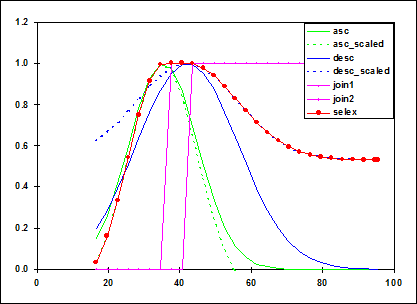
\includegraphics{DoubleNormal}
	\end{center}
	\caption{Contribution from each parameter in the overall shape of the double normal selectivity curve.}
	\label{fig:doublenormal}
\end{figure}

\myparagraph{Pattern 15 (size or age) - Mirror}
No parameters.  Whole age range is mirrored from another fleet. The mirrored selectivity pattern must have be from a lower fleet number (e.g., already specified before the mirrored fleet).

\myparagraph{Pattern 16 (age) - Gaussian (similar to Coleraine)}
	\begin{itemize}
		\item p1 – age below which selectivity declines
		\item p2 – scaling factor for decline
	\end{itemize}


\myparagraph{Pattern 9 (size) and 19 (age) - Simple Double Logistic}
	\begin{itemize}
		\item p1 – ascending inflection age/size
		\item p2 – ascending slope
		\item p3 – descending inflection age/size
		\item p4 – descending slope
		\item p5 – age or size at first selection; this is a specification parameter, so must not be estimated.  Enter integer that is age for pattern 19 and is bin number for pattern 9
		\item p6 – (0/1)  where a value of 0 causes the descending inflection to be a standalone parameter, and a value of 1 causes the descending inflection to be interpreted as an offset from the ascending inflection.  This is a specification parameter, so must not be estimated.
	\end{itemize}
A value of 1.0e-6 is added to the selectivity for all ages, even those below the minimum age.

\myparagraph{Pattern 25 (size) and 26 (age) - Exponential logistic}
	\begin{itemize}
		\item p1 – ascending rate, min: 0.02, max: 1.0, reasonable start value: 0.1.
		\item p2 – peak, as fraction of way between min size and max size.  Parameter min value:  0.01; max:  0.99; reasonable start value: 0.5.
		\item p3 – descending rate, min: 0.001, max: 0.5, reasonable start value:  0.01.  A value of 0.001 provides a nearly asymptotic curve. Values above 0.2 provide strongly dome-shaped function in which the p3 and p1 parameters interact strongly.
	\end{itemize}
	\begin{equation}
	\frac{e^{p3*p1(p2'-size)}}{1-p3(1-e^{p1(p2'-size)})}
	\end{equation}

\begin{figure}
	\begin{center}
		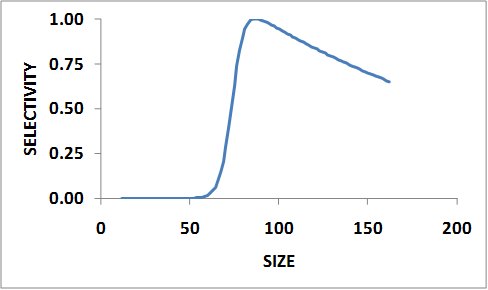
\includegraphics{ExpLogistic}
	\end{center}
	\caption{Example form of the exponential logistic selectivity with p1 = 0.30, p2 = 0.50, and p3 = 0.02.}
	\label{fig:explogistic}
\end{figure}

\myparagraph{Pattern 27 (size or age)- Cubic Spline}
This selectivity pattern uses the ADMB implementation of the cubic spline function. This function requires input of the number of nodes, the positions of those nodes, the parameter values at those nodes, and the slope of the function at the first and last node. In SS, the number of nodes is specified in the "special" column of the selectivity set-up.  The pattern number 27 is used to invoke cubic spline for size selectivity and for age selectivity; the input syntax is identical.
	
For a 3 node setup, the SS input parameters would be:
	\begin{itemize}
		\item p1 – 	code for initial set-up (0, 1 or 2) as explained below
		\item p2 – 	gradient at the first node (should be a small positive value)
		\item p3 – 	gradient at the last node (should be zero or a small negative value)
		\item p4-p6 – the nodes in units of cm; must be in rank order and inside of the range of the population length bins.  These must be held constant (not estimated, e.g., negative phase value) during a model run.
		\item  p7-p9 – the values at the nodes. Units are ln(selectivity).
	\end{itemize}

Notes:
	\begin{itemize}
		\item There must be at least 3 nodes.
		\item One of the node selectivity parameter values should be held constant so others are estimated relative to it.
		\item Selectivity is forced to be constant for sizes greater than the size at the last node.
		\item The overall selectivity curve is scaled to have a peak equal to 1.0.
		\item Terminal nodes cannot be at the min or max population length bins.
	\end{itemize}
	
Code for implementing cubic spline selectivity within SS can be found in \hyperlink{CubicSpline}{code examples}.

\begin{figure}
	\begin{center}
		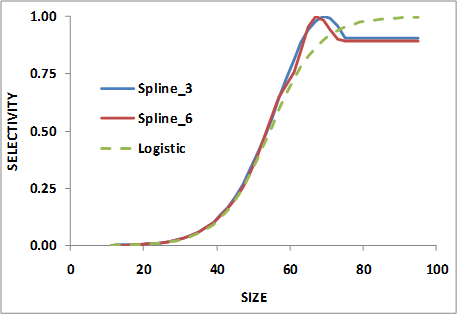
\includegraphics{CubicSpline}
	\end{center}
	\caption{Comparison between a 3 node and a 6 node cubic spline with a 2 parameter logistic function.  In fitting these functions, the 2 cubic spline approaches fit slightly better than the logistic, presumably because the data were slightly indicative of a small dome in selectivity.}
	\label{fig:cubicspline}
\end{figure}

	
Auto-Generation of Cubic Spline Control File Set-Up: A New SS feature pioneered with the cubic spline function is a capability to produce more specific parameter labels and to auto-generate selectivity parameter setup.  The auto-generation feature is controlled by the first selectivity parameter value for each fleet that is specified to use the cubic spline.  There are 3 possible values for this setup parameter:
	\begin{itemize}
		\item 0: no auto-generation, process parameter setup as read.
		\item 1: auto-generate the node locations based on the specified number of nodes and on the cumulative size distribution of the data for this fleet/survey.
		\item 2: auto-generate the nodes and also the min, max, prior, initial, and phase for each parameter.  
	\end{itemize}
	
With either the auto-generate option \#1 or \#2, it still is necessary to include in the parameter file placeholder rows of values so that the init\_matrix command can input the current number of values because all selectivity parameter lines are read as a single matrix dimensioned as N parameters x 14 columns.  The read values of min, max, initial, prior, prior type, prior stddev, and phase will be overwritten.
	
Cumulative size and age distribution is calculated for each fleet, summing across all samples and both sexes. These distributions are output in echoinput.sso and in a new OVERALL\_COMPS section of report.sso.
	
When the nodes are auto-generated, the first node is placed at the size corresponding to the 2.5\% percentile of the cumulative size distribution, the last is placed at the 97.5\% percentile of the size distribution, and the remainder are placed at equally spaced percentiles along the cumulative size distribution.  These calculated node values are output into control.ss\_new.  So, the user could extract these nodes from control.ss\_new, edit them to desired values, then, insert them into the input control file.  Remember to turn off auto-generation in the revised control file.
	
When the complete auto-generation is selected, the control.ss\_new would look like the table below:	

\begin{longtable}{p{1cm} p{1cm} p{1cm} p{2.9cm}  p{1.9cm}  p{4.2cm}}
	\hline
	LO \Tstrut & HI & INIT  &  <other entries> & Block Fxn & Parameter Label\Bstrut\\
	\hline
	\endfirsthead

	\hline
	LO \Tstrut & HI & INIT & <other entries> & Block Fxn & Parameter Label\Bstrut\\
	\hline
	\endhead

	0 \Tstrut &     2  &   2.0 & \multicolumn{1}{c}{...} & 0 & \#SizeSpline Code\\
	-0.001    & 	 1 &  0.13 & \multicolumn{1}{c}{...} & 0 & \#SizeSpline GradLo\\
	-1        & 0.001  & -0.03 & \multicolumn{1}{c}{...} & 0 & \#SizeSpline GradHi\\
	11        & 	95 & 	38 & \multicolumn{1}{c}{...} & 0 & \#SizeSpline Knot1\\
	11        & 	95 & 	59 & \multicolumn{1}{c}{...} & 0 & \#SizeSpline Knot2\\
	11        & 	95 & 	74 & \multicolumn{1}{c}{...} & 0 & \#SizeSpline Knot3\\
	-9        & 	 7 & 	-3 & \multicolumn{1}{c}{...} & 0 & \#SizeSpline Value1\\
	-9        &   	 7 & 	-1 & \multicolumn{1}{c}{...} & 0 & \#SizeSpline Value2\\
	-9        & 	 7 & -0.78 & \multicolumn{1}{c}{...} & 0 & \#SizeSpline Value3 \Bstrut\\
	\hline
\end{longtable}


\myparagraph{Pattern 41 (age) - Random Walk with User-Defined Scaling}
Selectivity pattern 17 with two additional parameters. The two additional parameters are the bin numbers to define the range of bins for scaling. All of the selectivity values will be scaled (divided) by the mean value over this range. The low and high bin numbers are defined before the other selectivity parameters.

	\begin{longtable}{p{1cm} p{1cm} p{1cm} p{2.9cm}  p{1.9cm}  p{4.2cm}}
		\hline
		LO \Tstrut & HI & INIT  &  <other entries> & Block Fxn & Parameter Label\Bstrut\\
		\hline
		\endfirsthead
	
		\hline
		LO \Tstrut & HI & INIT & <other entries> & Block Fxn & Parameter Label\Bstrut\\
		\hline
		\endhead

		0 & 20 & 10 & \multicolumn{1}{c}{...} & 0 & \#AgeSel\_ScaleAgeLo \Tstrut\\
		0 & 20 & 20 & \multicolumn{1}{c}{...} & 0 & \#AgeSel\_ScaleAgeHi \Bstrut\\
		\hline
	\end{longtable}


\myparagraph{Pattern 42 (size or age) - Cubic Spline with User-Defined Scaling}
Selectivity pattern 27 with two additional parameters. The two additional parameters are the bin numbers to define the range of bins for scaling. All of the selectivity values will be scaled (divided) by the mean value over this range. The low and high bin numbers are defined before the other selectivity parameters.

	\begin{longtable}{p{1cm} p{1cm} p{1cm} p{2.9cm}  p{1.9cm}  p{4.2cm}}
		\hline
		LO \Tstrut & HI & INIT  &  <other entries> & Block Fxn & Parameter Label\Bstrut\\
		\hline
		\endfirsthead
	
		\hline
		LO \Tstrut & HI & INIT & <other entries> & Block Fxn & Parameter Label\Bstrut\\
		\hline
		\endhead

		0 & 20 & 10 & \multicolumn{1}{c}{...} & 0 & \#AgeSpline\_ScaleAgeLo\Tstrut\\
		0 & 20 & 20 & \multicolumn{1}{c}{...} & 0 & \#AgeSpline\_ScaleAgeHi\Bstrut\\
		\hline
	\end{longtable}

\myparagraph{Pattern 43 (size) - Non-parametric with User-Defined Scaling}
Selectivity pattern 6 with two additional parameters. The two additional parameters are the bin numbers to define the range of bins for scaling. All of the selectivity values will be scaled (divided) by the mean value over this range. The low and high bin numbers are defined before the other selectivity parameters.
	
	\begin{longtable}{p{1cm} p{1cm} p{1cm} p{2.9cm}  p{1.9cm}  p{4.2cm}}
		\hline
		LO \Tstrut & HI & INIT  &  <other entries> & Block Fxn & Parameter Label\Bstrut\\
		\hline
		\endfirsthead
	
		\hline
		LO \Tstrut & HI & INIT & <other entries> & Block Fxn & Parameter Label\Bstrut\\
		\hline
		\endhead

		1 & 80 & 50 & \multicolumn{1}{c}{...} & 0 & \#SizeSel\_ScaleBinLo\Tstrut\\
		1 & 80 & 70 & \multicolumn{1}{c}{...} & 0 & \#SizeSel\_ScaleBinHi\Bstrut\\
		\hline
	\end{longtable}

\myparagraph{Pattern 44 (age)}
Similar to pattern 17 but with separate parameters for males and females. This selectivity pattern provides for a random walk in ln(selectivity).  In typical usage:
	\begin{itemize}
		\item p1 - First parameter (for age 0) could have a value of -1000 so that the age 0 fish would get a selectivity of 0.0.
		\item p2 - The first age for which mean selectivity = 1.
		\item p3 - The last age for which mean selectivity = 1.
		\item p4 - Male mean selectivity relative to the female selectivity mean entered as ln(ratio) for the male relative female selectivity.
		\item p5-p\textsubscript{n} - Additional parameter lines for the natural log of the selectivity change between ages corresponding to the user specified number of changes in the "special" column for the selectivity specification for each sex with females entered first then males.
		\item -999 input indicates to the model to keep the change unchanged from the previous age (keeps same rate of change).
		\item -1000 input indicates used only for male selectivity indicates to the model to set the change in male selectivity equal to the female change in selectivity.
	\end{itemize}
	
An example specification and setup for this selectivity option where selectivity is dome-shaped, peaking at age 2 with female and male selectivity are equal with 4 change points per sex:
	\begin{center}
		\begin{longtable}{p{1.5cm} p{1.5cm} p{1.5cm} p{1.5cm} }
			\hline
			\#Pattern & Discard & Male & Special\Tstrut\Bstrut\\
			\hline
			44 & 0 & 0 & 4 \Tstrut\Bstrut\\
			\hline
		\end{longtable}
	\end{center}

	\begin{longtable}{p{1cm} p{1cm} p{1cm} p{2.9cm}  p{1.8cm}  p{5.1cm}}
		\hline
		LO \Tstrut & HI & INIT  &  <other entries> & Block Fxn & Parameter Label\Bstrut\\
		\hline
		\endfirsthead
	
		\hline
		LO \Tstrut & HI & INIT & <other entries> & Block Fxn & Parameter Label\Bstrut\\
		\hline
		\endhead

		0     & 20 &  0     & \multicolumn{1}{c}{...} & 0 & \#first selex age \Tstrut\\
		0     & 20 &  2     & \multicolumn{1}{c}{...} & 0 & \#first age peak selex (mean) \\
		0     & 20 &  2     & \multicolumn{1}{c}{...} & 0 & \#last age peak selex (mean) \\
		-1    & 2  & -0.001 & \multicolumn{1}{c}{...} & 0 & \#male ln(ratio) \\
		-10   & 10 &  3.01  & \multicolumn{1}{c}{...} & 0 & \#female ln(selex) change 1\\
		-10   & 10 &  1.56  & \multicolumn{1}{c}{...} & 0 & \#female ln(selex) change 2\\
		-10   & 10 & -0.15  & \multicolumn{1}{c}{...} & 0 & \#female ln(selex) change 3\\
		-10   & 10 & -0.15  & \multicolumn{1}{c}{...} & 0 & \#female ln(selex) change 4\\
		-1000 & 10 & -1000  & \multicolumn{1}{c}{...} & 0 & \#male ln(selex) change 1\\
		-1000 & 10 & -1000  & \multicolumn{1}{c}{...} & 0 & \#male ln(selex) change 2\\
		-1000 & 10 & -1000  & \multicolumn{1}{c}{...} & 0 & \#male ln(selex) change 3\\
		-1000 & 10 & -1000  & \multicolumn{1}{c}{...} & 0 & \#male ln(selex) change 4\Bstrut\\
		\hline
	\end{longtable}
		
\myparagraph{Pattern 45 (age) - Revise Age}
Similar to pattern 14 but with separate parameters for males and females. Age-selectivity pattern 45 to allow selectivity-at-age to be the same as selectivity at the next younger age.  
	\begin{itemize}
		\item p1 - is the first age with non-zero selectivity.
		\item p2 - The first age in mean for peak selectivity
		\item p3 - The last age in mean for peak selectivity
		\item p4 - The male mean selectivity relative to the female mean, entered as ln(ratio) for the male relative female selectivity
		\item -999 input indicates to the model to keep the change unchanged from the previous age (keeps same rate of change).
		\item -1000 input indicates used only for male selectivity indicates to the model to set the change in male selectivity equal to the female change in selectivity.
	\end{itemize}
		
An example specification and setup for this selectivity option where selectivity is asymptotic, with female and male selectivity are equal with 4 change points per sex:
	\begin{center}
		\begin{longtable}{p{1.5cm} p{1.5cm} p{1.5cm} p{1.5cm} }
			\hline
			\#Pattern & Discard & Male & Special\Tstrut\Bstrut\\
			\hline
			45 & 0 & 0 & 3 \Tstrut\Bstrut\\
			\hline
		\end{longtable}
	\end{center}
		

	\begin{longtable}{p{1cm} p{1cm} p{1cm} p{2.9cm}  p{1.8cm}  p{5.1cm}}
		\hline
		LO \Tstrut & HI & INIT  &  <other entries> & Block Fxn & Parameter Label\Bstrut\\
		\hline
		\endfirsthead
		
		\hline
		LO \Tstrut & HI & INIT & <other entries> & Block Fxn & Parameter Label\Bstrut\\
		\hline
		\endhead

		0     & 20 &  2     &  \multicolumn{1}{c}{...} & 0 & \#first selex age \Tstrut\\
		0     & 20 &  5     &  \multicolumn{1}{c}{...} & 0 & \#first age peak selex (mean) \\
		0     & 20 &  5     &  \multicolumn{1}{c}{...} & 0 & \#last age peak selex (mean) \\
		-1    &  2 & -0.001 &  \multicolumn{1}{c}{...} & 0 & \#male ln(ratio) \\
		-10   & 10 & -8.1   &  \multicolumn{1}{c}{...} & 0 & \#female ln(selex) change 1\\
		-10   & 10 & -4.1   &  \multicolumn{1}{c}{...} & 0 & \#female ln(selex) change 2\\
		-10   & 10 & -1.8   &  \multicolumn{1}{c}{...} & 0 & \#female ln(selex) change 3\\
		-1000 & 10 & -1000  &  \multicolumn{1}{c}{...} & 0 & \#male ln(selex) change 1\\
		-1000 & 10 & -1000  &  \multicolumn{1}{c}{...} & 0 & \#male ln(selex) change 2\\
		-1000 & 10 & -1000  &  \multicolumn{1}{c}{...} & 0 & \#male ln(selex) change 3\Bstrut\\
		\hline
	\end{longtable}

\subsubsection{Retention}
Retention is defined as a logistic function of size or age.  It does not apply to surveys.  Four parameters (for asymptotic retention) or seven parameters (for dome-shaped retention) are used:
\begin{itemize}
	\item Asymptotic (4 parameters):
	\begin{itemize}
		\item p1 – ascending inflection,
		\item p2 – ascending slope,
		\item p3 – maximum retention controlling the height of the asymptote (smaller values result in lower asymptotes), often a time-varying quantity to match the observed amount of discard. As of v. 3.30.01, this parameter is now input in logit space ranging between -10 and 10. A fixed value of -999 would assume no retention of fish and a value of 999 would set asymptotic retention equal to 1.0,
		\item p4 – male offset to ascending inflection (arithmetic, not multiplicative),
	\end{itemize}
	\item Dome-shaped (add the following 3 parameters):
	\begin{itemize}
		\item p5 – descending inflection,
		\item p6 – descending slope, and
		\item p7 – male offset to descending inflection (arithmetic, not multiplicative).
	\end{itemize}
\end{itemize}

\begin{equation}
	\text{Retention} = \left(\frac{P3}{1 + e^{\frac{-(L-(P1+P4*male))}{P2}}}\right)*\left(1 - \frac{1}{1 + e^{\frac{-(L-(P5+P7*male))}{P6}}}\right)
\end{equation}

\subsubsection{Discard Mortality}
Discard mortality is defined as a logistic function of size such that mortality declines from 1.0 to an asymptotic level as fish get larger.  It does not apply to surveys and it does not affect the calculation of expected values for discard data.   It is applied so that the total mortality rate is:
\begin{center}
	dead fish = selectivity * (retain + (1.0-retain)*discard mortality)
\end{center}
If discard mortality is 1.0, all selected fish are dead; if discard mortality is 0.0, only the retained fish are dead.

Four parameters are used:
\begin{itemize}
	\item p1 – descending inflection
	\item p2 – descending slope
	\item p3 – maximum discard mortality
	\item p4 – male offset to descending inflection (arithmetic, not multiplicative)
\end{itemize}

Discard mortality is calculated as:
\begin{equation}
	\text{Discard Mortality} = \left(1 - \frac{1-P3}{1+e^{\frac{-(L-(P1+P4*male))}{P2}}}\right)
\end{equation}

\subsubsection{Sex-Specific Selectivity}
There are two approaches to specifying sex specific selectivity.  One approach allows male selectivity to be specified as a fraction of female selectivity (or vice versa).  This first approach can be used for any selectivity pattern.  The other option allows for separate selectivity parameters for each sex plus an additional parameter to define the scaling of one sex’s peak selectivity relative to the other sex’s peak.  This second approach has only been implemented for a few selectivity patterns.

\myparagraph{Male Selectivity as a Fraction of Female Selectivity (or vice versa):}
If the "domale" flag is set to 1, then the selectivity parameters define female selectivity and the offset defined below sets male selectivity relative to female selectivity.  The two sexes switch roles if the "domale" flag is set to 2.  Generally it is best to select the option so that the dependent sex has lower selectivity, thus obviating the need to rescale for selectivities that are greater than 1.0. Sex specific selectivity is done the same way for all size and age selectivity options.
\begin{itemize}
	\item p1 – size (age) at which a dogleg occurs (set to an integer at a bin boundary and do not estimate).
	\item p2 – ln(relative selectivity) at minimum length or age = 0.  Typically this will be set to a value of 0.0 (for no offset) and not estimated.  It would be a rare circumstance in which the youngest/smallest fish had sex-specific selectivity.
	\item p3 – ln(relative selectivity) at the dogleg.
	\item p4 – ln(relative selectivity) at maximum length or max age.
\end{itemize}

For intermediate ages, the natural log values are linearly interpolated on size (age).

If selectivity for the dependent sex is greater than the selectivity for the first sex (which always peaks at 1.0), then the male-female selectivity matrix is rescaled to have a maximum of 1.0.

\myparagraph{Male Selectivity Estimated as Offsets from Female Selectivity (or vice versa):}
A new sex selectivity option (3 or 4) has been implemented for size selectivity patterns 1 (logistic) and 23 and 24 (double normal) or age selectivity pattern 20 (double normal age).  Rather than calculate male selectivity as an offset from female selectivity, here the male selectivity is calculated by making the male parameters an offset from the female parameters (option 3), or females are offset from males with option 4.  The description below applies to option 3. If the size selectivity pattern is 1 (logistic), then read 3 parameters:
\begin{itemize}
	\item male parameter 1 is added to the first selectivity parameter (inflection)
	\item male parameter 2 is added to the second selectivity parameter (width of curve)
	\item male parameter 3 is the asymptotic selectivity
\end{itemize}

If the size selectivity pattern is 20, 23 or 24 (double normal), then:
\begin{itemize}
	\item male parameter 1 is added to the first selectivity parameter (peak)
	\item male parameter 2 is added to the third selectivity parameter (width of ascending side); then exp(this sum) per previous transform
	\item male parameter 3 is added to the fourth selectivity parameter (width of descending side); then exp(sum) per previous transform
	\item male parameter 4 is added to the sixth selectivity parameter (selectivity at final size bin); then 1/(1+exp(-sum)) per previous transform
	\item male parameter 5 is the apical selectivity for males
\end{itemize}

Note that the male selectivity offsets currently cannot be time-varying because they are offsets from female selectivity, they inherit the time-varying characteristics of the female selectivity.

\hypertarget{Dirichletparameter}{}
\subsubsection{Dirichlet Multinomial Error for Data Weighting}
If the Dirichlet multinomial error distribution was selected in the data file for either length or age data weighting an additional parameter line is required immediately following the selectivity parameter block. 
	
\begin{longtable}{p{1cm} p{1cm} p{1cm} p{2.9cm}  p{1.8cm}  p{6.5cm}}
	\multicolumn{6}{l}{The list of parameters to be read from the above setup would be:}\\
	\hline
	LO \Tstrut & HI & INIT  &  <other entries> & Block Fxn & Parameter Label\Bstrut\\
	\hline
	\endfirsthead
	
	\hline
	LO \Tstrut & HI & INIT & <other entries> & Block Fxn & Parameter Label\Bstrut\\
	\hline
	\endhead

	-5   & 10 & 0.5  & \multicolumn{1}{c}{...}  & 0   & \#ln(DM theta) Age or Length 1 \Tstrut\\
	-5   & 10 & 0.5  & \multicolumn{1}{c}{...}  & 0   & \#ln(DM theta) Age or Length 2\Bstrut\\
	\hline
\end{longtable}


\subsubsection{Selectivity Time-Varying Options}
The setup required for specifying time-varying options across parameter sections within SS (i.e., biology, recruitment, catchability, or selectivity) is the same and the basic description can be \hyperlink{tvOrder}{found above}. If time-varying selectivity parameters are invoked, short parameter lines are required to be read following the standard selectivity parameter section. If no selectivity parameters invoke any time-varying properties, this section is left blank (or completely commented out with \#).


\subsubsection{Two-Dimensional Auto-Regressive Selectivity}
A new experimental feature added within SS v.3.30.03.02. Earlier versions do not have this feature and hence this input is not expected.  This features allows for a matrix of auto-correlation selectivity deviations by age or length and time as described in \citet{xu_new_2019}. Unlike other options for time-varying selectivity in SS, these deviations are not in the selectivity parameters themselves, but exponential multipliers on whatever baseline selectivity has been chosen.  

When using this option for age-based selectivity, if there are not too many ages, a good choice for the baseline selectivity might be random walk selectivity (pattern 17) because it provides the most flexibility, allowing the deviations to be used only for the annual deviations around this baseline rather than the account for misspecification of the underlying functional form. Otherwise, a simple parametric selectivity form like logistic, exponential logistic, or double normal would be a better choices. This option has not yet been explored adequately to provide guidance on best practices.

\begin{longtable}{p{1cm} p{1cm} p{1cm} p{1.25cm} p{1.25cm} p{1.25cm} p{1.2cm} p{1.2cm} p{1cm} p{1cm} p{1cm}}
		
	\multicolumn{3}{l}{Typical Value} &  \multicolumn{8}{l}{Description and Options} \\
	\hline

	\multicolumn{3}{l}{1} & \multicolumn{8}{l}{Two-dimensional auto-regressive selectivity:}\Tstrut\\
	\multicolumn{3}{l}{ } & \multicolumn{8}{l}{0 = Not used,}\\
	\multicolumn{3}{l}{ } & \multicolumn{8}{l}{1 = Use 2D AR.}\Tstrut\\

	\multicolumn{11}{l}{COND = 1 Read the following long parameter lines:}\\
	\hline
	\Tstrut &    &      &      &      & Sigma & Use & Len(1)/ &       & Before & After\\
	Fleet & Ymin & Ymax & Amin & Amax & Amax  & Rho & Age(2)  & Phase & Range  & Range\Bstrut\\
	\hline
	   1    & 1979 & 2015 &  2   &  10  & 1     & 1   & 2       & 5     & 0   & 0\Tstrut\Bstrut\\
	\hline
	\\
	
	\multicolumn{11}{l}{continued:} \\
	\hline
	     &    &      &       & PRIOR & PRIOR &       &     & & & \Tstrut\\
	LO & HI & INIT & PRIOR & SD    & TYPE  & PHASE & \multicolumn{4}{l}{LABEL}\Bstrut\\
	\hline
	 0 & 4 & 1 & 1 & 0.1 & 6 & -4 & \multicolumn{4}{l}{\#Sigma selex}\Tstrut\\
	-1 & 1 & 0 & 0 & 0.1 & 6 & -4 & \multicolumn{4}{l}{\#Rho year}\\
	-1 & 1 & 0 & 0 & 0.1 & 6 & -4 & \multicolumn{4}{l}{\#Rho age}\Bstrut\\
	\multicolumn{11}{l}{\#Terminator line of 11 in length indicates the end of parameter input lines}\\
	-9999 & 1 & 1 & 1 & 1 & 1 & 1 & 1 & 1 & 1 & 1 \\
	\hline
\end{longtable}


Parameter Definitions:
\begin{itemize}
	\item Fleet: Fleet number to which semi-parametric deviations should be added.
	\item Ymin: First year with deviations.
	\item Ymax: Last year with deviations.
	\item Amin: First integer age (or population length bin index) with deviations.
	\item Amax: Last integer age (or population length bin index) with deviations.
	\item Sigma Amax: the last age (or population length bin index) for which a separate sigma should be read. For simplicity, it is easiest to set Sigma Amax equal to the Amin value which requires only a single sigma line (otherwise N = Sigma Amax - Amin input lines are required for the sigma parameters).
	\item Use Rho: Use autocorrelation parameters.
	\item Len(1) / Age(2): 1 or 2 to specify whether the deviations should be applied to length- or age-based selectivity.
	\item Phase: Phase to begin estimation of the deviation parameters.
	\item Before Range: How should selectivity be modeled in the years prior to Ymin? Available options are (0) apply no deviations, (1) use deviations from the first year with deviations (Ymin), and (3) use average across all years with deviations (Ymin to Ymax).
	\item After Range: Similar to Before Range but defines how selectivity should be modeled after Ymax.
\end{itemize}


\subsection{Tag Recapture Parameters}
Specify if tagging data are being used:


\begin{longtable}{p{1cm} p{1cm} p{1cm}  p{1.5cm}  p{2.9cm}  p{1.25cm}  p{4.25cm} }
	\hline
	\multicolumn{3}{l}{Typical Value} &  \multicolumn{4}{l}{Description and Options}\Tstrut\Bstrut\\
	\hline
	\multicolumn{3}{l}{1} &  \multicolumn{4}{l}{Tagging Data Present:} \Tstrut\\
	\multicolumn{3}{l}{}  &  \multicolumn{4}{l}{0 = No tagging data, or if tagging data is present in the data file, a value of 0} \\
	\multicolumn{3}{l}{}  &  \multicolumn{4}{l}{ here will auto-generate the tag parameter section in the control.ss\_new file.}\\
	\multicolumn{3}{l}{}  &  \multicolumn{4}{l}{1 = Read following lines of tagging data.} \Bstrut\\


	\multicolumn{7}{l}{COND = 1 Read the following long parameter lines:}\Tstrut\\
	\hline
	LO \Tstrut & HI & INIT & PRIOR &  <other entries> & Block Fxn & Parameter Label\Bstrut\\
	\hline
	\endfirsthead

	\hline
	LO \Tstrut & HI & INIT & PRIOR & <other entries> & Block Fxn & Parameter Label\Bstrut\\
	\hline
	\endhead

	\hline
	\endfoot
	\endlastfoot

	-10 & 10 & 9 & 9 & \multicolumn{1}{c}{...} & 0 & \#TG loss init 1\Tstrut\\
	-10 & 10 & 9 & 9 & \multicolumn{1}{c}{...} & 0 & \#TG loss chronic 1\\
	  1 & 10 & 2 & 2 & \multicolumn{1}{c}{...} & 0 & \#TG loss overdispersion 1\\
	-10 & 10 & 9 & 9 & \multicolumn{1}{c}{...} & 0 & \#TG report fleet 1\\
	 -4 &  0 & 0 & 0 & \multicolumn{1}{c}{...} & 0 & \#TG report decay 1\Bstrut\\
	 \hline
\end{longtable}

If there are multiple tagging groups or multiple fleets reporting tagged fish the additional needed parameter lines should be entered in order for each parameter type (i.e, TG loss init 1, TG loss init 2, TG loss chronic 1, TG loss chronic 2,..., TG report decay 1, TG report decay 2). 

Five parameter types are required for tagging data. Both the tag loss parameters and the reporting rate parameters are input as any real number and a logistic transformation is used to keep the resulting rates between 0 and 1:
\begin{itemize}
	\item Initial tag loss, representing fraction of tags that are shed or associated with tag-induced mortality immediately after tagging (1 parameter per tag group). 
	\item Chronic tag loss, representing annual rate of tag loss (1 parameter per tag group).
	\item Overdispersion parameter for the negative binomial likelihood associated with the total number of tag recaptures per tag group (1 parameter per tag group). This value represents the ratio of the variance to the mean of the distribution. As parameterized in ADMB, the likelihood is only defined for overdispersion parameters > 1, but a value of 1.001 will produce results essentially equal to those associated with a Poisson likelihood in which the variance is equal to the mean. This parameter is not transformed like the other 4 types.
	\item Initial reporting rate (1 parameter per fleet), the reporting rate of tags for a specific fleet.
	\item Reporting rate decay representing annual reduction in reporting rate (1 parameter per fleet).
\end{itemize}

The tagging reporting rate parameter is transformed within SS during estimation to maintain a positive value and is reported according to the transformation:
\begin{equation}
	\text{Tagging Reporting Rate} = \frac{e^{\text{input parameter}}}{1+e^{\text{input parameter}}}
\end{equation}

Currently, tag parameters cannot be time-varying.

A shortcoming was identified in the recapture calculations when using Pope's F Method and multiple seasons in SS versions prior to 3.30.14. The internal calculations were corrected in version 3.30.14. Now the Z-at-age is applied internally for calculations of fishing pressure on the population when using the Pope calculations.

\myparagraph{Mirroring of Tagging Parameters}
In version 3.30.14, the ability to mirror the tagging parameters from another tag group or fleet was added. With this approach, the user can have just one parameter value for each of the five tagging parameter types and mirror all other parameters. Note that parameter lines are still required for the mirrored parameters and only lower numbered parameters can be mirrored. Mirroring is evoked through the phase input in the tagging parameter section.  The options are:
\begin{itemize}
	\item No mirroring among tag groups or fleets: phase > -1000,
	\item Mirror the next lower (i.e., already specified) tag group or fleet: phase = -1000 and set other parameter values the same as next lower Tag Group or fleet,
	\item Mirror a lower (i.e., already specified) tag group of fleet x: phase = -100x and set other parameter values the same as the mirrored tag group or fleet( i.e., if you would like to mirror fleet 1 then the phase should -1001).
\end{itemize}

To avoid having to specify mirrored parameter lines, the tag parameters can be auto-generated. The control.ss\_new file created after running this model will have a full set of tagging parameter lines to use in future SS runs.

\hypertarget{GcompVar}{}
\subsection{Variance Adjustment Factors}
When doing iterative re-weighting of the input variance factors, it is convenient to do this in the control file, rather than the data file.  This section creates that capability.


\begin{longtable}{p{3cm} p{3cm} p{2.5cm} p{6.25cm} }

	\multicolumn{4}{l}{Read variance adjustment factors to be applied:}\\
	\hline
	Factor & Fleet & Value & Description \Tstrut\Bstrut\\
	\hline
	1 & 2 & 0.5 & \# Survey CV for survey/fleet 2 \Tstrut\\
	4 & 1 & 0.25 & \# Length data for fleet 1 \\
	4 & 2 & 0.75 & \# Length data for fleet 2\\
	-9999 & 0 & 0 & \# End read\Bstrut\\
	\hline
\end{longtable}


\myparagraph{Additive Survey CV - Factor 1}
The survey input variance (labeled survey CV) is actually the standard deviation of the ln(survey). The variance adjustment is added directly to this standard deviation. Set to 0.0 for no effect. Negative values are OK, but will crash if adjusted standard deviation value becomes negative.

\myparagraph{Additive Discard - Factor 2}	
The input variance is the CV of the observation. Because this will cause observations of near zero discard to appear overly precise, the variance adjustment is added to the discard standard deviation, not to the CV. Set to 0.0 for no effect.

\myparagraph{Additive Mean Body Weight - Factor 3}	
The input variance is in terms of the CV of the observation. Because such data are typically not very noisy, the variance adjustment is added to the CV and then multiplied by the observation to get the adjusted standard deviation of the observation.

\myparagraph{Multiplicative Length Composition - Factor 4}
The input variance is in terms of an effective sample size. The variance adjustment is multiplied times this sample size.  Set variance adjustment to 1.0 for no effect.

\myparagraph{Multiplicative Age Composition - Factor 5}
Age composition is treated the same way as length composition.
	
\myparagraph{Multiplicative Size-at-Age - Factor 6}	
Size-at-age input variance is the sample size for the N observations at each age.  The variance adjustment is multiplied by these N values. Set to 1.0 for no effect.
	
\myparagraph{Multiplicative Generalized Size Composition - Factor 7}	
Generalized size composition input variance is the sample size for each observation. The variance adjustment for each fleet is multiplied by these sample sizes. Set to 1.0 for no effect.
		
\myparagraph{Variance Adjustment Usage Notes}
The report.sso output file contains information in the "FIT\_LEN\_COMPS" and "FIT\_AGE\_COMPS"  useful for determining if an adjustment of these input values is warranted to better match the scale of the average residual to the input variance scale.
	
Because the actual input variance factors are modified, it is these modified variance factors that are used when creating parametric bootstrap data files. So, the control files used to analyze bootstrap generated data files should have the variance adjustment factors reset to null levels.


\hypertarget{Lambdas}{}
\subsection{Lambdas (Emphasis Factors)}
These values are multiplied by the corresponding likelihood component to calculate the overall negative log likelihood to be minimized.


\begin{tabular}{p{3cm} p{13cm}}
	\hline
	Typical Value & Description and Options\Tstrut\Bstrut\\
	\hline
	4 \Tstrut & Max lambda phase: read this number of lambda values for each element below.  The last lambda value is used for all higher numbered phases.\Bstrut\\
	1 & SD offset: \\
	  & 0 = The ln(like) to omit the + ln(s) term,\\
	  & 1 = The ln(like) to include the ln(s) term for CPUE, discard, growth CV, mean body weight, recruitment deviations. If you are estimating any variance parameters, SD offset must be set to 1.  \Bstrut\\
	\hline
\end{tabular}

\pagebreak

\myparagraph{Lambda Usage Notes}
\hypertarget{SaAlambda}{If} the CV for size-at-age is being estimated and the model contains mean size-at-age data, then the flag for inclusion of the + ln(stddev) term in the likelihood must be included. Otherwise, the model will always get a better fit to the mean size-at-age data by increasing the parameter for CV of size-at-age.

The reading of the lambda values has been substantially altered with SS v.3.30. Instead of reading a matrix containing all the needed lambda values, SS now just reads those elements that will be given a value other than 1.0.  After reading the datafile, SS sets lambda equal to 0.0 if there are no data for a particular fleet/data type, and a value of 1.0 if data exist. So beware if your data files had data but you had set the lambda to 0.0 in a previous version of SS.  First read an integer for the number of changes.


\begin{longtable}{p{3cm} p{3cm} p{2cm} p{3cm} p{3cm}}

	\multicolumn{5}{l}{Read the lambda adjustments by fleet and data type:}\\
	\hline
	Likelihood &       &       & Lambda & SizeFreq\Tstrut\\
	Component  & Fleet & Phase & Value  & Method \Bstrut\\
	\hline
	1 & 2 & 2 & 1.5 & 1 \Tstrut\\
	4 & 2 & 2 & 10 & 1 \\
	4 & 2 & 3 & 0.2 & 1 \\
	-9999 & 1 & 1 & 1 & 1 \Bstrut\\
	\hline
\end{longtable}


\begin{center}
	\begin{longtable}{ p{7.5cm} p{7.5cm} }
		\multicolumn{2}{l}{The codes for component are:}\\
		\hline
		1 = survey  				  & 10 = recruitment deviations \Tstrut\\	
		2 = discard 				  & 11 = parameter priors\\		
		3 = mean weight 			  & 12 = parameter deviations\\	
		4 = length 					  & 13 = crash penalty\\		
		5 = age 					  & 14 = morph composition\\
		6 = size frequency  		  & 15 = tag composition\\		
		7 = size-at-age 			  & 16 = tag negative binomial\\
		8 = catch 					  & 17 = F ballpark\\		
		9 = initial equilibrium catch & 18 = regime shift \Bstrut\\
		\hline
	\end{longtable}
\end{center}

\pagebreak

\subsection{Controls for Variance of Derived Quantities}
Additional standard deviation reported may be selected:

\begin{longtable}{p{1.1cm} p{1.4cm} p{1.2cm} p{1.2cm} p{1.3cm} p{1.6cm} p{1.4cm} p{1.4cm} p{1.4cm}}

	\hline
	\multicolumn{3}{l}{Typical Value} & \multicolumn{6}{l}{Description and Options}\Tstrut\Bstrut\\
	\hline
	\endfirsthead


	\multicolumn{3}{l}{0} & \multicolumn{6}{l}{0 = No additional std dev reporting;} \Tstrut\\
	\multicolumn{3}{l}{ } & \multicolumn{6}{l}{1 = read values below; and}\Bstrut\\
	\multicolumn{3}{l}{ } & \multicolumn{6}{l}{2 = read specification for reporting stdev for selectivity, size,numbers, and }\Bstrut\\
	\multicolumn{3}{l}{ } & \multicolumn{6}{l}{natural mortality.}\Bstrut\\
	\hline

\end{longtable}

COND = 1 or 2: Read the following lines (split into 3 rows for readability):
\begin{itemize}
	\item 4 values related to selectivity:
	\begin{enumerate}
		\item fleet number (or 0 if not used),
		\item type of selectivity to report: 1 = length, 2 = age, or 3 = combined (age with length),
		\item year, and
		\item number of bins to report, list entered below (note - combined will report in age bins).
	\end{enumerate}	
	\item 2 values related to growth:
	\begin{enumerate}
		\item growth pattern (or 0 if not used), and
		\item number of ages for reporting: list entered below (note - each sex will be reported).
	\end{enumerate}	
	\item 3 values related to numbers-at-age:
	\begin{enumerate}
		\item area (enter -1 for sum of all areas), or 0 for not used,
		\item year, and
		\item number of ages to report, list entered below (note - each sex will be reported and summed across growth patterns).
	\end{enumerate}
\end{itemize}

COND = 2, enter the above quantities plus:  
\begin{itemize}
	\item 2 additional values related to natural mortality-at-age:
	\begin{enumerate}
		\item growth pattern (or 0 for not used), and
		\item number of ages for reporting, list entered below (note - each sex will be reported).
	\end{enumerate}
\end{itemize}

Depending upon the entered options above subsequent conditional inputs may be need.
\begin{itemize}
	\item COND if selectivity specs number of bins to report > 0:
		\begin{itemize}
			\item Vector of bin indexes or -1 in first bin will overwrite entered vector with auto-generated list to cover logical range
	\end{itemize}
	\item COND if growth specs number of bins to report > 0 and empirical weight at age not used:
		\begin{itemize}
			\item … as for selectivity bins
		\end{itemize}
	\item COND if numbers-at-age specs number of ages > 0:
		\begin{itemize}
			\item … as for selectivity bins
		\end{itemize}
	\item COND == 2 and mortality-at-age specs number of ages > 0:
		\begin{itemize}
			\item … as for selectivity bins
		\end{itemize}
\end{itemize}


		
\begin{longtable}{p{1.1cm} p{1.4cm} p{1.2cm} p{1.2cm} p{1.3cm} p{1.6cm} p{1.4cm} p{1.4cm} p{1.4cm}}
	
	\hline
	\multicolumn{9}{l}{Example Input:}\Tstrut\Bstrut\\
	\hline
	
	\multicolumn{3}{l}{1} & \multicolumn{6}{l}{0 = No additional std dev reporting;} \Tstrut\\
	\multicolumn{3}{l}{ } & \multicolumn{6}{l}{1 = read values below; and}\Bstrut\\
	\multicolumn{3}{l}{ } & \multicolumn{6}{l}{2 = read specification for reporting stdev for selectivity, size,numbers, and }\Bstrut\\
	\multicolumn{3}{l}{ } & \multicolumn{6}{l}{natural mortality.}\Bstrut\\
	\hline
	
	\multicolumn{4}{l}{ 1 1 -1 5} & \multicolumn{5}{l}{\# Selectivity} \Bstrut\\
	\multicolumn{4}{l}{ 1 5}      & \multicolumn{5}{l}{\# Growth} \Bstrut\\
	\multicolumn{4}{l}{1 -1 5}    & \multicolumn{5}{l}{\# Numbers-at-age} \Bstrut\\

	\multicolumn{4}{l}{5 15 25 35 43} & \multicolumn{5}{l}{\# Vector with selectivity std bins (-1 in first bin to self-generate)}\Bstrut\\
	\multicolumn{4}{l}{1 2 14 26 40}  & \multicolumn{5}{l}{\# Vector with growth std ages picks (-1 in first bin to self-generate)}\Bstrut\\
	\multicolumn{4}{l}{1 2 14 26 40}  & \multicolumn{5}{l}{\# Vector with numbers-at-age std ages (-1 in first bin to self-generate)}\Bstrut\\
	 
		
	%\Tstrut Selex Type & Len/Age /Both & Year & Nselex Bins & Growth Pattern & N Growth Ages & NatAge Area & NatAge year  & N Natage\Bstrut\\
	%\hline
	%1 & 1 & -1 & 5 & 1 & 5 & 1 & -1 & 5\Tstrut\Bstrut\\ 
	
	%\hline
	%\multicolumn{9}{l}{Vector (length of 5) with selectivity std bin picks (-1 in first bin to self-generate).} \Tstrut\Bstrut\\
	%\hline
	%5 & 15 & 25 & 35 & 43 & & & & \Tstrut\Bstrut\\
	
	%\hline
	%\multicolumn{9}{l}{Vector (length of 5) with growth std bin picks (-1 in first bin to self-generate).} \Tstrut\Bstrut\\
	%\hline	
	%1 & 2 & 14 & 26 & 40 & & & & \Tstrut\Bstrut\\	
	
	%\hline
	%\multicolumn{9}{l}{Vector (length of 5) with NatAge std bin picks (-1 in first bin to self-generate).} \Tstrut\Bstrut\\
	%\hline	
	%1 & 2 & 14 & 26 & 40 & & & & \Tstrut\Bstrut\\
	
	\hline
	\bfseries{999} & \multicolumn{8}{l}{\#End of the control file input}\Tstrut\Bstrut\\
	\hline			
\end{longtable}



%Where:
%\begin{itemize}
%	\item Selex Type:  The index of the fleet to be output. 
%	\begin{itemize} 
%		\item 0 = No selectivity variance output; and
%		\item 1 = Selectivity variance output.
%	\end{itemize} 
	
%	\item Len/Age/Both:  
%	\begin{itemize}
%		\item 1 = Select length selectivity; 
%		\item 2 = Select age selectivity; and
%		\item 3 = Both length and age selectivity.
%	\end{itemize} 
	
%	\item Year:  
%	\begin{itemize}
%		\item year = Enter a value for the selected year; and
%		\item -1  = To get the selectivity in the end year.
%	\end{itemize} 

%	\item 	N Selex bins: enter the number of bins for which selectivity will be output. This number controls the number of items to be read below, even if the Selex Type is set to zero. In other words, the read occurs even if the effect of the read is disabled. 
	
%	\item Growth pattern: growth pattern is the number of the growth pattern to be output. Note that in a multiple season model, SS will output the size-at-age for the last birth season that gets any recruits within the year. Also, if growth parameters are not estimated, then standard deviation output of mean size-at-age is disabled. 
%	\begin{itemize}
%		\item positive value = Growth pattern,
%		\item 0 =  No variance output for size-at-age.   
%	\end{itemize}

%	\item 	N growth bins:  Number of ages for which size-at-age variance is requested.  This number controls the number of items to be read below, even if the growth pattern selection is set to zero.   In other words, the read occurs even if the effect of the read is disabled.
	
%	\item 	Area for Natage: specifies the area for which output of numbers at age is requested. 
%	\begin{itemize}
%		\item positive value = area to output;
%		\item 0 = Disables this output; and
%		\item -1 = Requests that numbers-at-age be summed across all areas.  In all cases, numbers-at-age is summed across all growth patterns and platoons and output for each sex.
%	\end{itemize}

%	\item 	NatAge Year:  specifies the year for which numbers-at-age are output.  
%	\begin{itemize}
%		\item year = The year to output; and
%		\item -1 = Requests output for year equal to end year + 1, hence the year that starts the forecast period.
%	\end{itemize}

%	\item N Natage bins: as with the N growth bins.
%\end{itemize}



\pagebreak